% Importamos el preámbulo con la configuración del documento
% Definición de la clase del documento
\documentclass[a4paper, 11pt]{book} % A4 paper and 11pt font size

% Entrada y salida de texto
\usepackage[T1]{fontenc}
\usepackage[utf8]{inputenc}
\usepackage[sfdefault]{roboto} % Option 'sfdefault' only if the base font of the document is to be sans serif

% Idioma
\usepackage[spanish, es-tabla]{babel} % Selecciona el español y el uso de la palabra "tabla" en lugar de "cuadro"

% Información reutilizable
\newcommand{\asunto}{Trabajo de Fin de Grado}
\newcommand{\titulo}{SmartU}
\newcommand{\tituloEng}{SmartU}
\newcommand{\subtitulo}{Desarrollo de un espacio colaborativo de ideas y proyectos}
\newcommand{\subtituloEng}{Development of a coworking space for ideas and projects}
\newcommand{\grado}{Grado en Ingeniería Informática}
\newcommand{\autor}{Juan José Jiménez García}
\newcommand{\email}{juanjojg@correo.ugr.es}
\newcommand{\tutor}{Miguel Gea Megías}
\newcommand{\escuela}{Escuela Técnica Superior de Ingenierías Informática y de Telecomunicación}
\newcommand{\departamento}{Departamento de Lenguajes y Sistemas Informáticos}
\newcommand{\universidad}{Universidad de Granada}
\newcommand{\ciudad}{Granada}
\providecommand{\keywords}{COMPLETAR ESTO}
\providecommand{\keywordsEng}{COMPLETE THIS}

% Otros paquetes importantes para el proyecto
\usepackage{url}
\usepackage{graphicx}
\usepackage{fancyhdr}
\usepackage{pdfpages}
\usepackage[hidelinks]{hyperref}

% Información del archivo
\hypersetup{
  pdfauthor = {\autor\ (\email)},
  pdftitle = {\titulo: \subtitulo},
  pdfsubject = {\asunto},
  pdfkeywords = {\keywords},
  pdfcreator = {LaTeX, con la distribución TeX Live},
  pdfproducer = {pdflatex}
}

% Modificación para que las páginas en blanco no tengan cabecera
\makeatletter
\def\clearpage{
  \ifvmode
    \ifnum \@dbltopnum =\m@ne
      \ifdim \pagetotal <\topskip
        \hbox{}
      \fi
    \fi
  \fi
  \newpage
  \thispagestyle{empty}
  \write\m@ne{}
  \vbox{}
  \penalty -\@Mi
}
\makeatother

% Definición del estilo de las cabeceras
\pagestyle{fancy}
\fancyhf{}
\fancyhead[LO]{\leftmark}
\fancyhead[RE]{\rightmark}
\fancyhead[RO,LE]{\textbf{\thepage}}
\setlength{\headheight}{1.5\headheight}

% Redefinición de comandos
\renewcommand{\chaptermark}[1]{\markboth{\textbf{#1}}{}}
\renewcommand{\sectionmark}[1]{\markright{\textbf{\thesection. #1}}{}}
% \renewcommand{\lstlistingname}{Fragmento de código}
% \renewcommand{\lstlistlistingname}{Índice de fragmentos de código}

% Creación de comandos
% \newcommand{\HRule}{\rule{\linewidth}{0.5mm}}
% \newcommand{\bigrule}{\titlerule[0.5mm]}

% Ajuste para minimizar el fragmentado de listados
% \lstnewenvironment{listing}[1][]
%   {\lstset{#1}\pagebreak[0]}{\pagebreak[0]}


\begin{document}

% Portada del documento
\begin{titlepage}

\newlength{\centeroffset}
\setlength{\centeroffset}{-0.5\oddsidemargin}
\addtolength{\centeroffset}{0.5\evensidemargin}

\noindent\hspace*{\centeroffset}

\begin{minipage}{\textwidth}

\centering


\includegraphics[width=0.9\textwidth]{logo_ugr}\\[1.4cm]

\textsc{\Large\asunto\\[0.2cm]}
\textsc{\grado}\\[1cm]

{\Huge\bfseries\titulo\\}
\noindent\rule[-1ex]{\textwidth}{3pt}\\[3.5ex]
{\large\bfseries\subtitulo}

\end{minipage}

\vspace{1.5cm}
\noindent\hspace*{\centeroffset}

\begin{minipage}{\textwidth}

\centering

\textbf{Autor}\\{\autor}\\[2.5ex]
\textbf{Tutor}\\{\tutor}\\[1.5cm]


\includegraphics[width=0.3\textwidth]{logo_etsiit}\\[0.1cm]

\textsc{\escuela}\\
\textsc{---}\\
\ciudad, \today\\

\end{minipage}

\end{titlepage}


% Prefacio del documento
\cleardoublepage
\thispagestyle{empty}

\begin{center}
{\LARGE\bfseries\titulo: \subtitulo}\\
\end{center}
\begin{center}
\autor
\end{center}

\bigskip
\noindent{\textbf{Palabras clave}: \textit{\keywords}\\

\section*{Resumen}
Este documento detalla mi trabajo y participación en el proyecto multidisciplinar llevado a cabo en la Universidad de Granada.\\

\textbf{SmartU} nace del trabajo en equipo realizado por un grupo de estudiantes y sus tutores, como respuesta a un problema habitual de la vida universitaria, que es el fomento de proyectos de carácter multidisciplinar.\\

Lo que se pretende con este trabajo es crear una plataforma basada en un formato de \textbf{red social} que permita a los estudiantes publicar proyectos e ideas y con ello encontrar a otros estudiantes de diversas disciplinas que quieran unirse para llevar a cabo la idea.\\

SmartU pretende ser un apoyo y una forma de fomentar más el \textbf{trabajo en equipo}, algo que la sociedad actual demanda mucho en sus puestos de trabajo y que no termina de fraguar del todo en las universidades. \\

Como resultado de este trabajo, también se obtienen una serie de \textbf{resultados y conclusiones} sobre cómo ha sido este primer ``proceso piloto'' de equipo multidisciplinar, que servirá de ayuda para mejorar en el futuro los problemas encontrados.

\cleardoublepage
\thispagestyle{empty}

\begin{center}
{\LARGE\bfseries\tituloEng: \subtituloEng}\\
\end{center}
\begin{center}
\autor
\end{center}

\bigskip
\noindent{\textbf{Keywords}: \textit{\keywordsEng}\\

\section*{Abstract}
This final degree document explains my work and collaboration on the multidisciplinary project made on the University of Granada.\\

\textbf{SmartU} is the result of the teamwork carried out by a group of students and their tutors in response to a common problem in the university life, which is the promotion of multidisciplinary projects.\\

This work aims to create a \textbf{social network based} web platform which allows students to publish projects and ideas in order to find another students from other specialties who want to join to carry it out.\\

SmartU is meant to be a support to promote \textbf{work in team}, since it's something highly required by today's jobs but it's not very popular in universities.\\

As a result from this project, we also got a bunch of \textbf{results and conclusions} about how well this first multidisciplinary project was, which will be used to improve in the future the found problems.

\chapter*{}
\thispagestyle{empty}

\noindent\rule[-1ex]{\textwidth}{2pt}\\[4.5ex]

Yo, \textbf{\autor}, alumno de la titulación \textbf{\grado} de la \textbf{\escuela} de la \textbf{\universidad}, con DNI 76655977J, autorizo la ubicación de la siguiente copia de mi Trabajo de Fin de Grado en la biblioteca del centro para que pueda ser consultada por las personas que lo deseen.

\vspace{6cm}

\noindent \textbf{Fdo: \autor}

\vspace{2cm}

\begin{flushright}
\ciudad, a \today
\end{flushright}

\chapter*{}
\thispagestyle{empty}

\noindent\rule[-1ex]{\textwidth}{2pt}\\[4.5ex]

D. \textbf{\tutor}, profesor del \textbf{\departamento} de la \textbf{\universidad}.

\vspace{0.5cm}

\textbf{Informa:}

\vspace{0.5cm}

Que el presente trabajo, titulado \textit{\textbf{\titulo: \subtitulo}}, ha sido realizado bajo su supervisión por \textbf{\autor}, y autoriza la defensa de dicho trabajo ante el tribunal que corresponda.

\vspace{0.5cm}

Y para que conste, expide y firma el presente informe en \ciudad, a \today.

\vspace{1cm}

\textbf{El tutor:}

\vspace{5cm}

% \begin{figure}[H]
% \includegraphics[width=0.3\textwidth]{firma_tutor}
% \end{figure}

\noindent\textbf{\tutor}

\chapter*{Agradecimientos}
\thispagestyle{empty}

\vspace{1cm}

Quisiera agradecer a mi familia todo el apoyo que me han brindado no solo durante mi etapa en la universidad, sino también en el colegio y el instituto. Gracias por toda vuestra ayuda y cariño. \\

Gracias a mis amigos y amigas de la ETSIIT de Granada, los mejores compañeros de trabajo que he conocido y con quienes he pasado momentos geniales. \\

A mis profesores, tanto a los buenos como a los ``no tan buenos'', les agradezco que me hayan ayudado a ser quien soy hoy con su atención y esfuerzo por querer transmitir sus valiosos conocimientos. \\

Y a mis compañeros del TFG, con quienes he compartido estos últimos meses dando forma a este proyecto, muchas gracias. Especialmente a Emilio, y a mi tutor Miguel.


\frontmatter
\begingroup
\let\cleardoublepage\clearpage
  \tableofcontents
  % \listoffigures
  % \listoftables
  % \lstlistoflistings
\endgroup

\newpage
\thispagestyle{empty}

% Capítulos del documento
\mainmatter
\chapter{Introducción}

Prueba de capítulo.

\chapter{Metodología de trabajo multidisciplinar}
\label{ch:metodologia}

\section{El trabajo en equipo}
Este proyecto multidisciplinar quiere poner en práctica el mismo concepto sobre el que trabaja: \textit{Gestión de equipos de trabajo multidisciplinares para desarrollo de proyectos}. Aquí entran en juego varios conceptos importantes vistos en el apartado \ref{sec:objetivos} de objetivos:

\begin{itemize}
    \item Por un lado nos encontramos con el reto de \textbf{crear} una plataforma para gestionar proyectos multidisciplinares, facilitando la tarea de encontrar a personas para formar equipo y que trabajen en una idea.
    \item Por otro lado, nosotros mismos como equipo, debemos trabajar en la organización para que todo salga adelante y podamos desarrollar dicha plataforma.
\end{itemize}

Esto nos sirve de \textbf{experiencia} sobre cómo es el trabajo en equipo multidisciplinar. Ayudará a encontrar \textbf{debilidades y fortalezas}, y servirá para que los productos que creemos sean mejores y sean de utilidad ante la problemática del trabajo en equipo.\\

En el nacimiento de este equipo, se planteó que debemos funcionar de forma similar a una Startup \cite{startup}. Siguiendo esa lógica, trabajamos sobre una idea innovadora para resolver un problema complejo, empleando la tecnología para llegar a cumplir el objetivo.\\

Sobre el concepto de la plataforma SmartU, nacen una serie de \textbf{líneas de trabajo} que consideramos importantes para lograr un producto completo y útil para su público objetivo, por ello es necesario que se trabaje en ellas de forma correcta.

\begin{description}
    \item[Software] La línea de trabajo donde crear aplicaciones web y móviles que el público objetivo usará con el fin de facilitar la tarea de la creación de proyectos multidisciplinares.
    \item[Marketing] Esta línea de trabajo concentra sus esfuerzos en la búsqueda de formas de promoción adecuadas al público y que garanticen que SmartU llegue al máximo número de personas posibles. Destacamos por ejemplo el uso de las redes institucionales ya existentes para dar difusión, así como la creación de redes sociales propias de la plataforma como forma de acercamiento a los demás.
    \item[Diseño gráfico] La identidad visual es el reto al que se enfrenta esta línea de trabajo. Se ha de encontrar un estilo y diseño diferenciador que además sea agradable al usuario, y que de alguna forma represente los conceptos sobre los que trabajamos, como por ejemplo el concepto principal de ciudades inteligentes.
    \item[Plan de empresa] El plan de empresa tiene como objetivo encontrar una estrategia de negocio que sirva para que esta \textit{startup} sea viable en el futuro.
\end{description}

\subsection{Mi trabajo}
Mi ocupación se centra en la línea de trabajo de \textbf{Software}. Como estudiante de Ingeniería Informática, mi ocupación sería la de crear la plataforma web de SmartU, donde el público objetivo pueda registrarse y subir sus propuestas de proyecto, establecer criterios para encontrar a los estudiantes de las disciplinas que necesitan, y recibir valoraciones y opiniones del resto de usuarios, todo siguiendo en la medida de lo posible un enfoque de red social que haga el uso de la aplicación más ``humano'' y no tanto el de usar una máquina donde publicas tu idea y esperas que te aparezcan candidatos.

\section{Integrantes del equipo}
El equipo de trabajo se ha compuesto de diferentes \textbf{profesores y estudiantes} de diversas disciplinas de la universidad. Podemos ver su nombre y ocupación en la \textbf{tabla \ref{miembrossmartu}}. Todos hemos aportado conocimientos de nuestro campo al proyecto para intentar lograr los mejores resultados, recibiendo opiniones y puntos de vista muy diferentes que ayudan y complementan.\\

\begin{table}
    \begin{center}
        \begin{tabular}{|p{4.5cm}|p{6.5cm}|}
            \hline
                \rowcolor{Gray}\multicolumn{1}{|c|}{\textbf{Integrante}}
                & \multicolumn{1}{|c|}{\textbf{Ocupación}} \\
            \hline
                Juan Árbol Gutiérrez & Estudiante de CC.EE. y Empresariales \\
            \hline
                Irene Castillo Pardo & Estudiante de Comunicación y Audiovisuales \\
            \hline
                Emilio Chica Jiménez & Estudiante de Ingeniería Informática \\
            \hline
                Victoria Guerra Molina & Estudiante de Comunicación y Audiovisuales \\
            \hline
                Juan José Jiménez García & Estudiante de Ingeniería Informática \\
            \hline
                Javier Labrat Rodríguez & Estudiante de Ingeniería Informática \\
            \hline
                Germán Zayas Cabrera & Estudiante de Bellas Artes \\
            \hline
                Miguel Gea Megías & Profesor de Ingeniería Informática \\
            \hline
                Guillermo Maraver Tarifa & Profesor de CC.EE. y Empresariales \\
            \hline
                Alejandro Grindlay Moreno & Profesor de Ingeniería Civil \\
            \hline
        \end{tabular}
        \caption{Integrantes del proyecto multidisciplinar SmartU}
        \label{miembrossmartu}
    \end{center}
\end{table}

El equipo no se componía de estas personas exactas al comienzo. A lo largo del curso \textbf{fueron incorporándose} más compañeros, lo cual también suponía un reto, por el hecho de gestionar ese cambio no previsto para adaptar todo.\\

Cada uno de los miembros del equipo tenía asignado un rol o tarea. Era importante que cada uno se dedicase a algo relacionado con sus conocimientos, de esta manera se esperaba conseguir mejores resultados, al \textbf{delegar en la persona adecuada la tarea adecuada}. Podemos ver el reparto de roles en la \textbf{tabla \ref{rolessmartu}}.\\

\begin{table}
    \begin{center}
        \begin{tabular}{|p{5cm}|p{6cm}|}
            \hline
                \rowcolor{Gray}\multicolumn{1}{|c|}{\textbf{Integrante/s}}
                & \multicolumn{1}{|c|}{\textbf{Rol o tarea}} \\
            \hline
                Juan Árbol Gutiérrez & Emprendedor y gestor de estrategia empresarial \\
            \hline
                Juan José Jiménez García & Gestor de proyecto y desarrollador de software \\
            \hline
                Emilio Chica Jiménez & Gestor tecnológico y desarrollador de software \\
            \hline
                Irene Castillo Pardo y Victoria Guerra Molina & Gestoras de audiovisuales \\
            \hline
                Germán Zayas Cabrera & Diseñador gráfico \\
            \hline
                Javier Labrat Rodríguez, Miguel Gea Megías, Guillermo Maraver Tarifa y Alejandro Grindlay Moreno & Tutores y consultores para dudas \\
            \hline
        \end{tabular}

        \caption{Integrantes del proyecto multidisciplinar SmartU}
        \label{rolessmartu}
    \end{center}
\end{table}

En la \textbf{tabla \ref{tareassmartu}} se puede ver un resumen general del trabajo realizado por cada uno de los miembros del equipo, o que va a realizar más adelante.

\newpage
\begin{longtable}{|m{4.5cm}|m{6.5cm}|}
    \hline
        \rowcolor{Gray}\multicolumn{1}{|c|}{\textbf{Integrante}}
        & \multicolumn{1}{|c|}{\textbf{Aportaciones}} \\
    \hline
        Juan Árbol Gutiérrez & \begin{itemize}
            \item Organizador del Design Thinking y Brainstorming
            \item Creador del plan estratégico de empresa
            \item Responsable de realización de entrevistas a posibles usuarios objetivo del sistema
            \item Presentador del proyecto en la Facultad de Ciencias de la Actividad Física y del Deporte
        \end{itemize} \\
    \hline
        Irene Castillo Pardo & \begin{itemize}
            \item Colaborador en el Design Thinking y Brainstorming
            \item Creadora del video de presentación del proyecto
            \item Creación del making of del proyecto
        \end{itemize} \\
    \hline
        Emilio Chica Jiménez & \begin{itemize}
            \item Creador de la aplicación móvil del proyecto
            \item Organizador del Design Thinking y Brainstorming
            \item Moderador de seminario de tecnologías emergentes
            \item Gestor de reuniones
        \end{itemize} \\
    \hline
        Victoria Guerra Molina & \begin{itemize}
            \item Colaborador en el Design Thinking y Brainstorming
            \item Investigadora de una campaña de difusión del proyecto en redes sociales y medios de publicidad
        \end{itemize} \\
    \hline
        Juan José Jiménez García & \begin{itemize}
            \item Organizador del Design Thinking y Brainstorming
            \item Gestor del proyecto
            \item Creador de la aplicación web
            \item Coordinador y documentador de reuniones
            \item Coordinador del repositorio de archivos y calendario
        \end{itemize} \\
    \hline
        Javier Labrat Rodríguez & \begin{itemize}
            \item Presentador del proyecto en la Facultad de Ciencias de la Actividad Física y del Deporte
            \item Creador de un proyecto que servirá de muestra para nuestro sistema SmartU
        \end{itemize} \\
    \hline
        Germán Zayas Cabrera & \begin{itemize}
            \item Colaborador en el Design Thinking y Brainstorming
            \item Creador de la identidad visual del proyecto
            \item Creador del diseño de la página web de presentación del proyecto
        \end{itemize} \\
    \hline
        Miguel Gea Megías & \begin{itemize}
            \item Creador de la idea original
            \item Agrupador de los miembros del equipo
            \item Consejero para el desarrollo del proyecto
            \item Colaborador en el Design Thinking y Brainstorming
            \item Gestor de las reuniones
        \end{itemize} \\
    \hline
        Guillermo Maraver Tarifa & \begin{itemize}
            \item Colaborador en el Design Thinking y Brainstorming
            \item Consejero de Juan para el desarrollo del proyecto
            \item Consejero de marketing y promoción del proyecto
        \end{itemize} \\
    \hline
        Alejandro Grindlay Moreno & \begin{itemize}
            \item Colaborador en el Design Thinking y Brainstorming
            \item Consejero para el desarrollo del proyecto
        \end{itemize} \\
    \hline
    \caption{Aportaciones de los miembros del equipo}\label{tareassmartu}\\
\end{longtable}

\subsection{Dependencias entre miembros del equipo}
Una de las cosas que tuvimos en cuenta al principio fue que, en un proyecto multidisciplinar, es muy importante \textbf{encontrar sinergias} entre los miembros del mismo, es decir, encontrar puntos comunes que permitan una colaboración fructuosa entre dos personas. Así, el trabajo que teníamos que hacer cada uno se vería más reforzado al contar con el punto de vista y la ayuda proporcionada por otra persona de diferente disciplina.\\

Así, nos encontramos con los siguientes ejemplos de tareas en las que hemos encontrado sinergias (es decir, que gracias a la colaboración mutua, creemos que el resultado obtenido es mejor que haberlo hecho sin su ayuda):

\begin{itemize}
    \item La propia \textbf{implementación de las plataformas} colaborando con mi compañero Emilio consiguió que el software propuesto presentara una funcionalidad más rica y completa que haberlo hecho por separado.
    \item Germán aportó sinergias en casi todas las líneas de trabajo, ya que su tarea (\textbf{diseño de la identidad corporativa}) es aplicable no solo al software, sino también al marketing.
    \item Entre Germán y Juan hubo colaboración para confeccionar el diseño de la \textbf{página web de presentación del proyecto}, así como la creación de sus contenidos.
    \item Javier, con su proyecto ya terminado, sirvió como \textbf{prueba de concepto}, al permitir incorporar su proyecto al futuro sistema que se va a diseñar para demostrar al público objetivo las capacidades de SmartU.
\end{itemize}

Pero también es cierto que hubo ciertos problemas a lo largo del curso que impidieron la aprición de más sinergias. Principalmente los problemas fueron la falta de tiempo para que algunos miembros pudieran hacer sus tareas, y la tardía definición de todos los conceptos del proyecto y la necesidad de la aplicación móvil, que en un principio no quedaba clara cual podía ser tu utilidad y diferenciación.\\

Esta experiencia nos hace ver que este tipo de proyectos requieren de más dedicación de la que se pensaba. Al ser una primera experiencia piloto, no teníamos del todo claro lo que podía pasar, pero ello nos servirá para que en los años siguientes el proceso mejore.

\section{Gestión del trabajo}
Como encargado de gestionar el proyecto además de realizar software, junto con Miguel llevamos a cabo la \textbf{organización del trabajo} con el objetivo de conseguir la mayor agilidad posible para la comunicación y para documentar los progresos. En las siguientes secciones de este apartado se describe con más detalle lo que se ha realizado para cada uno de los puntos de gestión.

\subsection{Comunicación}
Un proyecto de esta índole necesitaba de varias \textbf{reuniones}, donde poder debatir asuntos y tomar decisiones, así como para realizar ciertas técnicas creativas de generación de ideas y establecer las funcionalidades de los productos a desarrollar. Estos puntos son tratados más adelante en esta documentación.\\

Las reuniones tuvieron lugar en diferentes puntos de encuentro de todos los campus de la Universidad de Granada, siendo el más habitual el de la Facultad de Ciencias Económicas y Empresariales, debido a la disponibilidad de mejores salas de reunión y trabajo en equipo.\\

Debido a la diferencia de disciplinas que presentaban los integrantes, se hacía necesario establecer un \textbf{horario semanal} donde se cuadrase la disponibilidad de todos los miembros para que estuviera el máximo número posible en las reuniones. Dicho horario se actualizaba semana a semana según las necesidades de los integrantes.

Podemos describir el \textbf{proceso de organización de reuniones} de la siguiente manera:

\begin{enumerate}
    \item Como gestión previa a una reunión, ocurría lo siguiente:
    \begin{enumerate}
        \item Se \textbf{comunicaba a los gestores} la necesidad de realizar una reunión para tratar un asunto importante del proyecto.
        \item Los gestores se \textbf{reunían} para establecer los puntos de la próxima reunión.
        \item Se \textbf{comunicaba al resto del equipo} de la necesidad de realizar la reunión y se les pedía que indicasen en el horario los días que mejor le convenían, para encontrar el punto común donde pudieran ir todos.
        \item Los profesores, debido a la posibilidad que presentan de \textbf{reservar salas de reuniones} más adecuadas que los que los estudiantes tenían permitido, se encargaban de encontrar sitio para celebrar la reunión en base a la disponibilidad de los asistentes.\\
        También se encargaban de asegurarse de que la sala que se fuera a reservar contase con material adecuado para la reunión, como un \textbf{proyector, pizarra}, etc.
        \item Se establecía en el calendario oficial del proyecto (con \textbf{Google Calendar} \cite{googlecalendar}) y se informaba al resto del equipo por el medio correspondiente.
    \end{enumerate}
    \item Al comenzar la reunión, se resumían los puntos tratados en la \textbf{reunión anterior}, a modo de recordatorio y para aquellos miembros que no hubieran podido asistir a dicha reunión. Tras el resumen, se procede a informar de los puntos a debatir en la reunión actual.
    \item Al acabar la reunión se comentan los \textbf{nuevos puntos a tratar} de cara a la próxima reunión, y se anotan para no olvidarlos y que los gestores puedan prepararlos.
    \item El gestor del proyecto crea un \textbf{acta de reunión} donde se detallan los puntos debatidos y se apuntan los temas a tratar para la próxima reunión.
\end{enumerate}

Como detalle final de la gestión de la comunicación, en la tabla \ref{canalescomunicacion} se puede ver las valoraciones dadas tras su uso a los distintos canales de comunicación que utilizamos entre los miembros del equipo.

\begin{table}
    \begin{center}
        \begin{tabular}{|l|p{3cm}|p{5cm}|}
            \hline
                \rowcolor{Gray}\multicolumn{1}{|c|}{\textbf{Canal}}
                & \multicolumn{1}{|c|}{\textbf{Utilidad}} & \multicolumn{1}{|c|}{\textbf{Valoración}} \\
            \hline
                E-mail & Usado en las primeras semanas & No es recomendable, debido a que no siempre se comprueba el correo electrónico con regularidad y no se sabe si alguien lo ha leido. \\
            \hline
                WhatsApp \cite{whatsapp} & Utilizado durante todo el proyecto & Aplicación de mensajería más utilizada, respuesta casi inmediata y mayor rapidez de comunicación. \\
            \hline
                Slack \cite{slack} & Utilizado al final del proyecto & Es una plataforma muy utilizada por empresas y equipos de desarrollo, con numerosas funcionalidades de comunicación entre miembros que agilizan bastante la comunicación. \\
            \hline
        \end{tabular}

        \caption{Canales de comunicación empleados y valoración de los mismos}
        \label{canalescomunicacion}
    \end{center}
\end{table}

\subsection{Documentación}
Para gestionar la documentación y todo el contenido que el equipo fuese produciendo a lo largo del tiempo, se hacía necesario contar con un espacio común de alojamiento de archivos. Para esto se optó por utilizar \textbf{Google Drive} \cite{googledrive}, un servicio de almacenamiento de archivos en la nube rápido y sencillo de utilizar que todos los miembros del equipo conocían.\\

Todos tenían acceso a dicho directorio online, y ahí se iban dejando los documentos que generábamos, como pueden ser:
\begin{itemize}
    \item Presentaciones para exponer en reuniones.
    \item Actas de reuniones.
    \item Bocetos de diseño de aplicaciones o de identidad visual.
    \item Calendario semanal actualizado.
\end{itemize}

\section{Resultados}
Tras la realización de los \textbf{seminarios de tecnologías emergentes y técnicas de creatividad}, se procedió a realizar una sesión de \textit{Brainstorming} y un proceso creativo de \textit{Design Thinking} para que todos aportaran ideas y conceptos que nos servirían para dar forma a nuestro sistema a desarrollar. En el anexo \ref{sec:designthinking} podrá encontrar una \textbf{lista de todas las ideas} que se obtuvieron, clasificadas de la siguiente manera:

\begin{itemize}
    \item Ideas
    \item Objetivos
    \item Limitaciones
    \item Aspectos positivos
\end{itemize}

Más adelante se realizó otra sesión de Design Thinking debido a que hubo algunas ausencias en la primera reunión, y sirvió para \textbf{afianzar todo lo visto} en la primera y proceder con ello al desarrollo del producto software, que se detalla en el capítulo \ref{ch:desarrollo}.\\

En el anexo \ref{sec:actas} puede encontrar disponible las actas de reunión realizadas durante este primer año de vida del proyecto.

\chapter{Proceso de desarrollo}
\label{ch:desarrollo}

En este tercer capítulo comenzaremos por una introducción para explicar la forma de trabajo que se ha seguido, seguido del apartado de análisis, en el que definimos qué es lo queremos que sea exactamente SmartU, pasando por el diseño de la aplicación web habiendo conocido ya los actores del sistema y sus requisitos.\\

A continuación pasamos al apartado de implementación, donde se detalla de forma más técnica cómo se ha creado este sistema de información web, y terminamos hablando de la fase de pruebas. El capítulo incluye un apartado de herramientas que han sido utilizadas para el desarrollo.

\section{Introducción}
Al comenzar el desarrollo del proyecto, se pudo apreciar que había una alta posibilidad de sufrir cambios a lo largo del proceso debido a que el alcance del mismo no estaba muy delimitado. Es por ello que se optó por seguir una metodología principalmente ágil, la cual permitía mayor flexibilidad y facilidad para adaptar posibles cambios.\\

En el desarrollo ágil es importante la comunicación entre todos los miembros del equipo y que éstos, de alguna forma, participen activamente durante el desarrollo. No todos los miembros de este equipo multidisciplinar trabajan en el ámbito de la Ingeniería Informática, pero sabíamos que podían colaborar en las primeras fases aportando ideas y posibles requisitos. Sin embargo, sí que era importante que hubiera comunicación y consenso entre los miembros del área de Informática. Con mi compañero Emilio se realizó una puesta en común para intentar unificar las plataformas que cada uno teníamos que desarrollar.\\

Siguiendo algunos de los principios del desarrollo ágil, se ha evitado realizar documentación innecesaria, y se ha optado por ir a lo primordial y esencial, sin que ello repercuta en la calidad del software. Hay que tener en cuenta que este desarrollo pretende ser continuado y mejorado en el tiempo, por lo que una documentación base correcta es más importante que rellenar páginas y páginas innecesarias.\\

Por último, añadiremos que se ha preferido optar por establecer una lista de requisitos del sistema en lugar de emplear la técnica de las \textbf{historias de usuario}, ya que no son de obligado cumplimiento el desarrollarlas, y se ha de tener en cuenta el hecho de que el desarrollo será continuado por otras personas en el futuro.

\section{Análisis}
La fase de análisis se distribuye en \textbf{dos grandes bloques}:

\begin{itemize}
    \item El primer bloque comprende el análisis en equipo del problema y la extracción de unos primeros requisitos y usuarios base sobre los que basaremos nuestras decisiones futuras a la hora de desarrollar el sistema. Aquí se realizarán diversas técnicas de generación de ideas y prototipado para acotar y definir mejor el sistema.
    \item El segundo bloque es más habitual del proceso de desarrollo de software, ya que se va a dedicar a recopilar y mostrar los requisitos del sistema ya definidos correctamente, tras haber terminado el análisis del primer bloque.
\end{itemize}

\subsection{Generación de ideas y extracción de requisitos}
El equipo de trabajo multidisciplinar se reunió varias veces para realizar sesiones de generación de ideas, tales como el \textit{Brainstorming}, que llevó a cabo mi compañero Emilio, o el proceso creativo de \textit{Design Thinking} llevado a cabo por mi compañero Juan y por mí.\\

Más adelante se obtuvo más información gracias a la presentación del proyecto multidisciplinar que se hizo en la Facultad de Ciencias de la Actividad Física y del Deporte, realizada por los compañeros Javier y Juan. Allí se pudo enseñar el proyecto a potenciales usuarios (\textit{stakeholders}) y recibimos opiniones muy interesantes de posibles características que les gustaría ver para que fuese una aplicación web más completa y funcional.

\subsubsection{Usuarios del sistema}
Tras las reuniones de generación de ideas, se llegó a la siguiente conclusión respecto a \textbf{quiénes son los usuarios potenciales del sistema}. Es importante poder definir a los posibles futuros usuarios de nuestra aplicación para así poder enfocar mejor los requisitos y el diseño de nuestra aplicación web. Nuestro equipo en si consta de algunos de ellos: son los estudiantes y profesores, o en general, la comunidad educativa.

\begin{itemize}
    \item Los \textbf{estudiantes} son potenciales usuarios registrados de nuestra aplicación web. Podemos concretar más e irnos al segmento de estudiantes de último año de grado o máster que necesitan una idea para realizar un proyecto de final de grado/máster, pero también están aquellos estudiantes que cuentan con una idea para un proyecto y necesitan a otros estudiantes con los que conformar un equipo.\\
    Este grupo de usuarios es el que se prevee que sería el que utilizase el sistema con mayor frecuencia.
    \item Otro segmento de usuarios es los \textbf{habitantes de la ciudad}. La diferencia radica en que por lo general, es un colectivo no asociado a la universidad y desconocedor de lo que ocurre dentro de ésta. Por ello, no son considerados potenciales usuarios que se van a registrar en el sistema, pero si entrarán y consultarán las ideas que se han publicado.\\
    Pueden ser participantes activos de un proyecto que se esté creando si éste es un proyecto que le interese o afecte a su entorno (barrio, movilidad, economía, etc).
    \item Por último, tenemos el grupo de \textbf{usuarios empresarios}. Estos son aquellas personas que, o bien tienen una idea, o encuentran interesante una idea que han visto publicada en la aplicación. Pueden ponerse en contacto con un equipo de un proyecto y ayudarles con financiación o promoción de su idea, entre otras posibilidades.
\end{itemize}

Para representar de una forma más visual a estos usuarios, se han creado una serie de bocetos de usuario (o \textit{User Persona}), que esquematizan y ayudan a definir de un vistazo el tipo de perfil de usuario que hemos definido. Podemos verlos en las figuras \ref{usuario_estudiante}, \ref{usuario_ciudadano} y \ref{usuario_empresario}.\\

Como podemos ver, el conjunto de potenciales usuarios intenta abarcar a todo el conjunto de la población, por lo que una buena implantación del mismo podría \textbf{reportar enormes beneficios} para todos ellos, ya sea encontrando un proyecto en el que trabajar, como llevar a cabo una idea que mejore la vida en general de los ciudadanos.

\begin{figure}
    \centering
    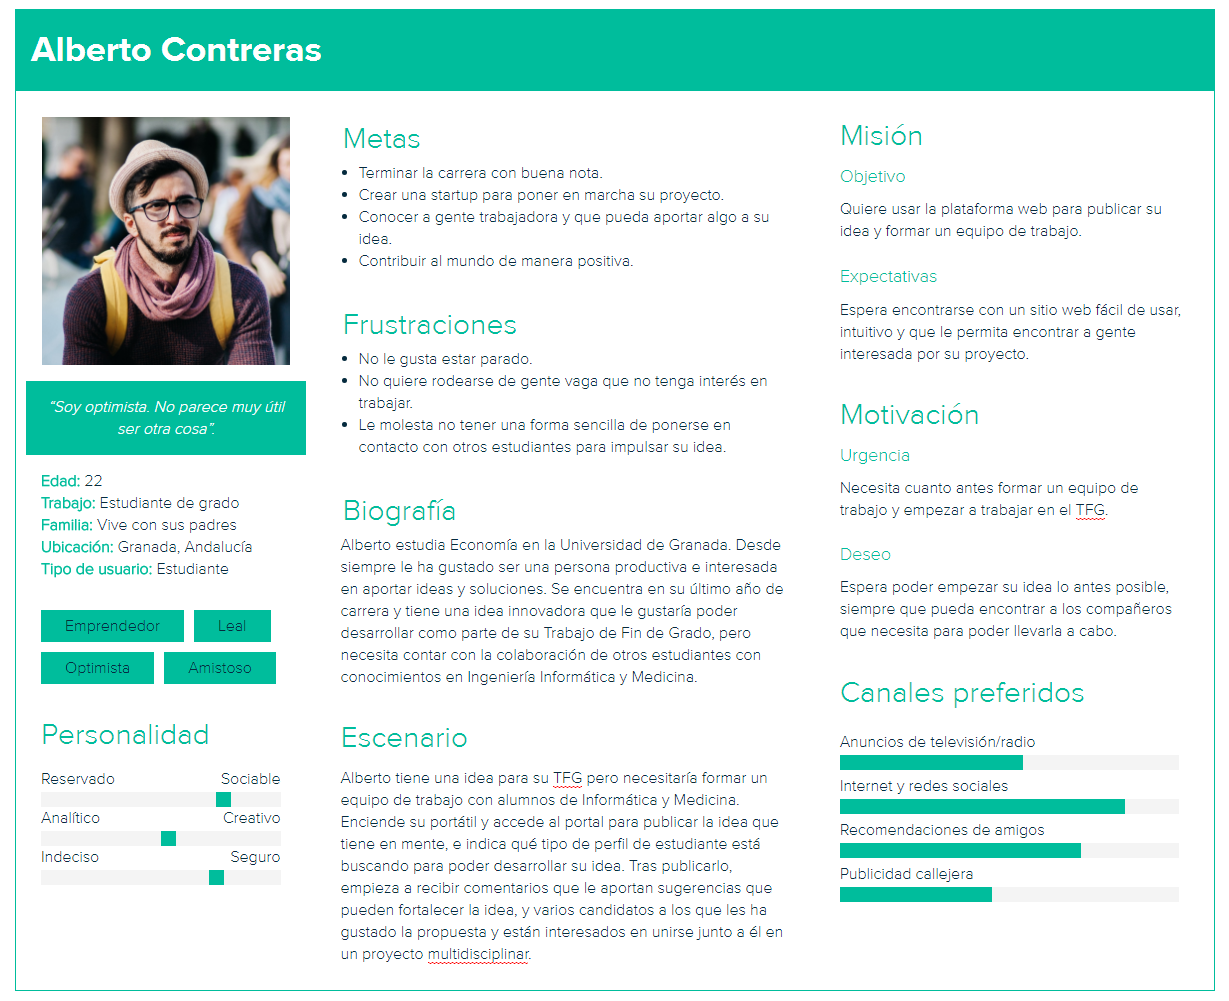
\includegraphics[width=\textwidth]{usuario_estudiante}
    \caption{\textit{User Persona} de un estudiante}
    \label{usuario_estudiante}
\end{figure}

\begin{figure}
    \centering
    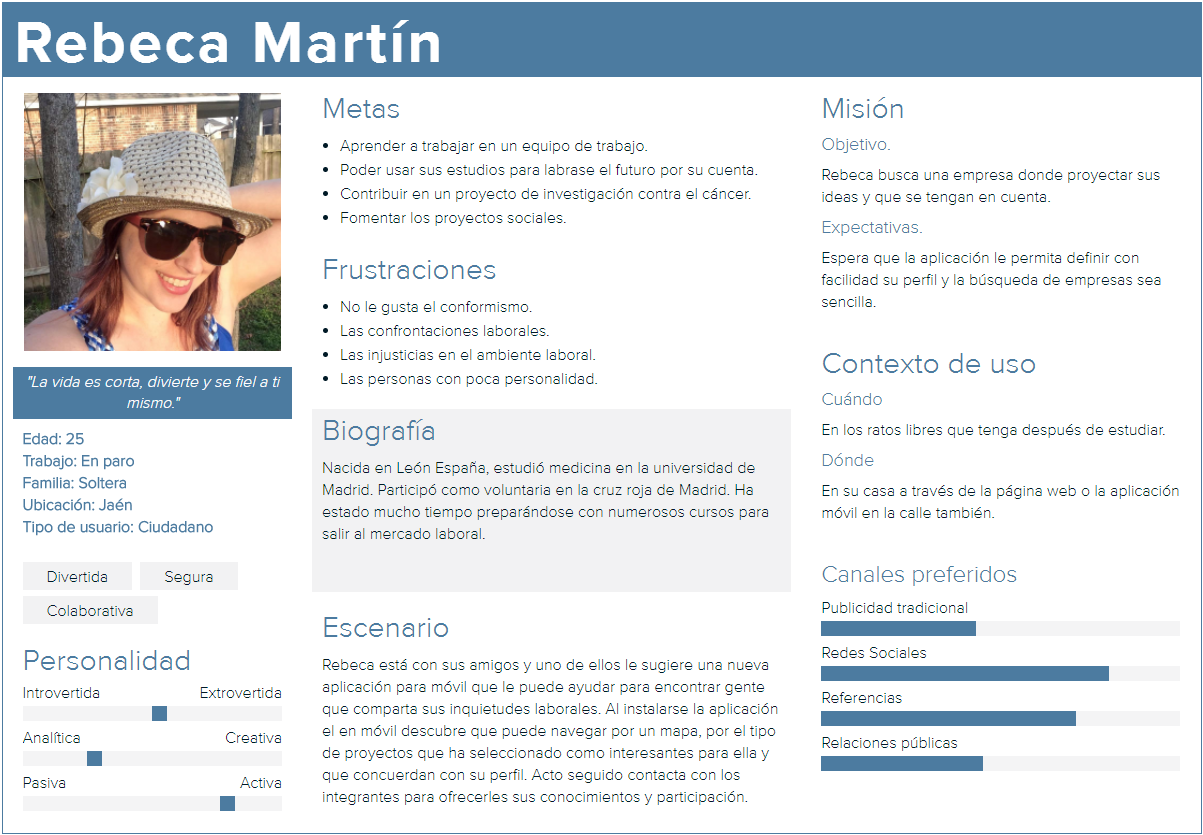
\includegraphics[width=\textwidth]{usuario_ciudadano}
    \caption{\textit{User Persona} de un ciudadano}
    \label{usuario_ciudadano}
\end{figure}

\begin{figure}
    \centering
    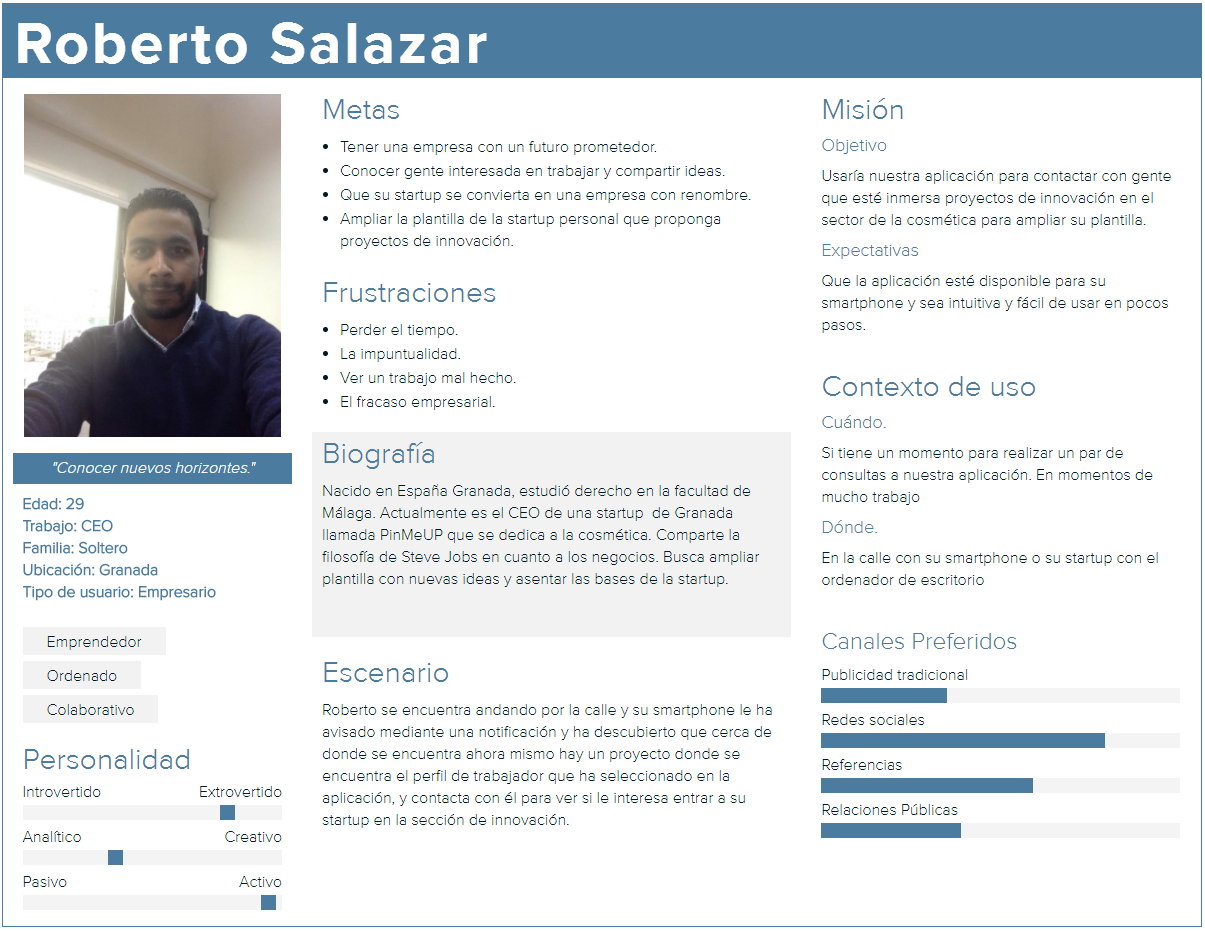
\includegraphics[width=\textwidth]{usuario_empresario}
    \caption{\textit{User Persona} de un empresario}
    \label{usuario_empresario}
\end{figure}

\subsection{Requisitos del sistema}
En base a todas las reuniones e información recabada de las mismas y de posibles stakeholders, se ha confeccionado la siguiente lista de requisitos del sistema.

\subsection*{Requisitos de datos}
Se quiere implementar un sistema de información basado en web que sea capaz de almacenar la información relativa a proyectos para la universidad, permitiendo la asignación de información más detallada como área de conocimiento del proyecto, descripción y avances del mismo, así como la información perteneciente a los usuarios que se registren en la plataforma, sus comentarios e información de perfil.

\begin{description}
    \item[RD1. Proyecto:] Un proyecto necesita almacenar la siguiente información:
        \begin{description}
            \item[Nombre:] Cadena de caracteres.
            \item[Descripción:] Cadena de caracteres.
            \item[Página web:] Cadena de caracteres.
            \item[Localización:] Cadena de caracteres.
            \item[Coordenadas:] Cadena de caracteres.
            \item[Fecha de creación:] Fecha de alta del proyecto en el sistema.
            \item[Fecha de eliminación:] Fecha estimada de finalización del proyecto.
            \item[Fecha de actualización:] Fecha de última actualización del proyecto.
            \item[Propietario:] Identificador del usuario registrado que creó el proyecto.
        \end{description}
    \item[RD2. Redes sociales:] Los proyectos y los usuarios pueden definir sus propias redes sociales para darse a conocer, y necesitan la siguiente información:
        \begin{description}
            \item[Nombre:] Cadena de caracteres.
            \item[URL:] Cadena de caracteres.
            \item[ID de usuario:] Identificador del usuario.
            \item[ID del proyecto:] Identificador del proyecto.
        \end{description}
        Una red social petenece a un usuario o a un proyecto, se han unificado para evitar redundancia.
    \item[RD3. Área del proyecto:] Los proyectos tienen una o varias áreas, y se necesita la siguiente información para poder guardarlas.
        \begin{description}
            \item[Nombre:] Cadena de caracteres.
            \item[Descripción:] Cadena de caracteres.
        \end{description}
    \item[RD4. Buena Idea:] Una buena idea se asemeja a un ``Me gusta'' de redes como Facebook o Twitter. Necesita la siguiente información:
        \begin{description}
            \item[ID del proyecto:] Identificador del proyecto.
            \item[ID del usuario:] Identificador del usuario.
        \end{description}
    \item[RD5. Especialidad:] La especialidad es algo a lo que un usuario se dedica o que tiene experiencia en ello. Sirve para encontrar a gente de un determinado campo que necesita un proyecto. Se necesita la siguiente información:
        \begin{description}
            \item[Nombre:] Cadena de caracteres.
            \item[Descripción:] Cadena de caracteres.
        \end{description}
    \item[RD6. Experiencia en especialidad:] Partiendo del requisito de dato anterior, un usuario cuenta con un cierto nivel de experiencia en una especialidad, lo cual requiere almacenar la siguiente información:
        \begin{description}
            \item[Experiencia:] Cadena de caracteres.
            \item[ID de la especialidad:] Identificador de la especialidad.
            \item[ID del usuario:] Identificador del usuario.
        \end{description}
    \item[RD7. Comentario:] Los usuarios registrados pueden dejar comentarios en sus proyectos o en los de otros usuarios. Se necesita la siguiente información:
        \begin{description}
            \item[Contenido:] Cadena de caracteres.
            \item[Fecha de creación:] Fecha insertada cuando se creó el comentario.
            \item[ID del usuario:] Identificador del usuario que hace el comentario.
            \item[ID del proyecto:] Identificador del proyecto donde se comenta.
        \end{description}
    \item[RD8. Avance:] Un proyecto puede tener un conjunto de avances que muestre a los usuarios el progreso que se está logrando con el proyecto. Necesita la siguiente información:
        \begin{description}
            \item[Nombre:] Cadena de caracteres.
            \item[Descripción:] Cadena de caracteres.
            \item[Fecha de creación:] Fecha de publicación del avance
            \item[Imagen destacada:] Cadena de caracteres del nombre de un archivo de imagen.
            \item[ID del proyecto:] Identificador del proyecto al que va asociado.
        \end{description}
    \item[RD9. Vacante:] Una vacante representa una disponibilidad de un puesto, en una determinada disciplina, como integrante en un proyecto. Se necesita la siguiente información:
        \begin{description}
            \item[Experiencia:] Una cadena de caracteres.
            \item[Especialidad:] Un identificador de una especialidad concreta.
        \end{description}
    \item[RD10. Hashtag:] Uno o varios proyectos pueden tener etiquetas conocidas como \textit{hastags}, y se necesita guardar para ello:
        \begin{description}
            \item[Nombre:] Una cadena de caracteres.
        \end{description}
    \item[RD11. Usuario:] Un usuario necesita almacenar la siguiente información:
        \begin{description}
            \item[Nombre:] Cadena de caracteres.
            \item[Apellidos:] Cadena de caracteres.
            \item[Email:] Cadena de caracteres.
            \item[Contraseña:] Cadena de caracteres.
            \item[Biografía:] Cadena de caracteres.
            \item[Página web:] Cadena de caracteres.
            \item[Localización:] Cadena de caracteres.
            \item[Puntos:] Número entero.
            \item[CIF:] Cadena de caracteres.
            \item[Admin:] Booleano.
            \item[Verificado:] Booleano.
            \item[Avatar:] Cadena de caracteres del nombre de un archivo de imagen.
        \end{description}
    \item[RD12. Solicitud colaboración:] Los usuarios pueden solicitar colaborar en un proyecto que tenga vacantes disponibles. Se necesita almacenar la siguiente información:
        \begin{description}
            \item[Fecha:] Fecha de creación de la solicitud.
            \item[Descripción:] Una cadena de caracteres.
            \item[Usuario solicitante:] Identificador del usuario que solicita colaborar.
            \item[Proyecto solicitado:] Identificador del proyecto en el que se desea colaborar.
        \end{description}
    \item[RD13. Colaborador:] Un usuario puede ser colaborador de un proyecto en una determinada especialidad. Se necesita almacenar:
        \begin{description}
            \item[ID del usuario:] Identificador del usuario colaborador.
            \item[ID del proyecto:] Identificador del proyecto donde colabora.
            \item[ID de especialidad:] Identificador de la especialidad del colaborador.
        \end{description}
    \item[RD14. Intereses:] Los usuarios pueden marcar intereses en determinadas áreas. Para ello se necesita guardar:
        \begin{description}
            \item[ID del usuario:] Identificador del usuario que marca un interés.
            \item[ID del área:] Identificador del área donde el usuario marca un interés.
        \end{description}
    \item[RD15. Status:] Un ususario puede tener un status en base a su participación en la aplicación web, por ejemplo publicando proyectos o bien dando ``Buena Idea'' a otros. Se requiere la siguiente información:
        \begin{description}
            \item[Nombre:] Cadena de caracteres. Es el nombre que recibe el status.
            \item[Puntos:] Número entero que representa los puntos que se han de alcanzar para llegar a dicho status.
        \end{description}
    \item[RD16. Seguidor:] Un usuario puede seguir a otro para estar al tanto de sus proyectos y de lo que hace en la aplicación web. Se necesita almacenar lo siguiente:
        \begin{description}
            \item[ID del usuario seguido:] Identificador del usuario al que se sigue.
            \item[ID del usuario seguidor:] Identificador del usuario que está siguiendo.
        \end{description}
\end{description}

\subsection*{Restricciones semánticas}
\begin{description}
    \item[RS1.] Un usuario no registrado no puede participar en la aplicación web salvo para consultar la información.
    \item[RS2.] Un usuario no puede tener el mismo email o nombre de usuario que otro registrado anteriormente.
    \item[RS3.] Un proyecto solo puede tener un usuario propietario.
    \item[RS4.] Los usuarios solo pueden modificar o eliminar proyectos de los que son propietarios.
    \item[RS5.] Un usuario puede solicitar unirse al proyecto si hay vacantes y si no es ya propietario o colaborador.
    \item[RS6.] Un usuario no puede seguirse a sí mismo.
    \item[RS7.] Un usuario no puede dar Buena Idea a su/s propio/s proyecto/s.
    \item[RS8.] Los usuarios con correo corporativo reconocido serán registrados automáticamente como usuarios ``verificados''.
\end{description}

\subsection*{Requisitos funcionales}
\subsubsection{Requisitos funcionales de inserción}
\begin{description}
    \item[RF1. Registrar usuario:] un usuario invitado puede registrarse en el sistema para poder utilizar el resto de funcionalidades.
    \item[RF2. Crear proyecto:] Un usuario registrado puede crear un nuevo proyecto en el sistema para dar a conocer su idea.
    \item[RF3. Dar Buena Idea:] Un usuario puede dar un Buena Idea a un proyecto
    \item[RF4. Dejar un comentario:] Un usuario registrado puede dejar un comentario en un proyecto.
    \item[RF5. Elegir áreas de interés:] Un usuario registrado puede seleccionar una o más áreas que sean de su interés para encontrar proyectos afines.
    \item[RF6. Seguir a un usuario:] Un usuario registrado en el sistema puede seguir a otro usuario para estar al tanto de su actividad en la aplicación.
    \item[RF7. Crear vacante:] Un usuario propietario de un proyecto puede crear una vacante para buscar colaboradores para su proyecto.
    \item[RF8. Solicitar colaboración:] Un usuario puede solicitar colaborar en un proyecto que no sea suyo si éste tiene una vacante disponible.
    \item[RF9. Insertar avance:] Un usuario propietario de un proyecto puede crear un avance de un proyecto que muestre algun tipo de progreso.
    \item[RF10. Insertar nuevo colaborador:] Un usuario propietario de un proyecto puede aceptar o rechazar una petición de colaboración para una vacante.
\end{description}

\subsubsection{Requisitos funcionales de consulta}
\begin{description}
    \item[RF11. Listar solicitudes:] Un usuario propietario de un proyecto puede listar las solicitudes de colaboración en su proyecto pendientes de aprobación.
    \item[RF12. Listar vacantes:] Cualquier usuario puede listar las vacantes existentes para un proyecto.
    \item[RF13. Listar avances:] Cualquier usuario puede listar los avances realizados en un proyecto.
    \item[RF14. Listar proyectos:] Cualquier usuario puede listar los proyectos existentes en la aplicación.
    \item[RF15. Listar usuarios:] Cualquier usuario puede listar usuarios registrados en la aplicación.
    \item[RF16. Listar comentarios:] Cualquier usuario puede listar los comentarios de un proyecto.
    \item[RF17. Listar áreas:] Cualquier usuario puede listar las áreas disponibles en el sistema.
    \item[RF18. Listar colaboradores:] Cualquier usuario puede listar los colaboradores actuales de un proyecto.
    \item[RF19. Consultar detalles de un proyecto:] Cualquier usuario puede ver los detalles de un proyecto.
    \item[RF20. Consultar detalles de un usuario:] Cualquier usuario puede ver el perfil de otro usuario registrado en la aplicación.
\end{description}

\subsubsection{Requisitos funcionales de eliminación}
\begin{description}
    \item[RF21. Eliminar áreas de interés:] Un usuario registrado puede modificar su perfil y eliminar una o varias áreas que sean de su interés.
    \item[RF22. Eliminar Buena Idea de un proyecto:] Un usuario puede eliminar el Buena Idea que le ha dado a un proyecto.
    \item[RF23. Dejar de seguir a un usuario:] Un usuario registrado puede dejar de seguir a otro usuario registrado en el sistema.
\end{description}

\subsection*{Requisitos no funcionales}
\begin{description}
    \item[RNF1.] La aplicación web debe estar finalizada para septiembre de 2017.
    \item[RNF2.] La aplicación web debe tener un diseño adaptable a todo tipo de tamaños de pantalla de dispositivo.
    \item[RNF3.] La aplicación web debe funcionar correctamente en la mayoría de navegadores de Internet más utilizados y en sus últimas versiones disponibles.
    \item[RNF4.] El código de la aplicación debe estar correctamente comentado para facilitar la tarea de mejorarlo a los futuros desarrolladores que continúen el proyecto.
\end{description}

\section{Diseño}


\section{Implementación}
Tras el proceso de análisis de nuestro sistema y extracción de los requisitos que necesitaría nuestra aplicación web (\textit{expuestos en anteriores apartados de este capítulo}), en este voy a detallar los principales aspectos de la implementación de la misma, incidiendo en aspectos importantes e inherentes al proceso de desarrollo de un sistema de información web.\\

La codificación de la aplicación web de SmartU venía condicionada por la necesidad de un desarrollo que fuese agilizado e iterativo, intentando completar funcionalidades específicas en cada \textit{``paso''} que se diese a lo largo de este proceso. Esto me llevó a tomar una serie de decisiones respecto al lenguage de programación que utilizaría, así como el conjunto de herramientas que me ayudarían con esta tarea, pero siempre teniendo como máxima un desarrollo correcto y bien realizado.

\subsection{Laravel}
¿Por qué utilizar un \textit{``framework''} de desarrollo web como Laravel? La elección del mismo no fue fácil, y llevó algo de tiempo debido al análisis de pros y contras que podría encontrarme a lo largo del proceso de desarrollo. Existen numerosos lenguages de programación como Python, JavaScript, Java, etc, todos con diferentes soluciones de desarrollo web. En el caso de Laravel, se basa en el lenguage PHP, que es ya bien conocido en el mundo de la programación web, y a lo largo de los años ha ido mejorando su potencial con nuevas versiones que incorporaban características que si estaban presentes en otros lenguages.\\

Laravel es un framework de desarrollo web basado en PHP creado por Taylor Otwell en el año 2011. Fue creado con el intento de proporcionar una alternativa más avanzada a \textbf{CodeIgniter}. En muchos lugares de Internet, Laravel es conocido por darle un muy necesitado lavado de cara a PHP, y hacerlo de nuevo más atractivo a la vista de los desarrolladores.\\

Laravel agiliza los procesos en casi todos los apartados existentes del desarrollo de una aplicación web. Proporciona un conjunto de herramientas para gestionar la autenticación de usuarios, bases de datos rutas, entre otros elementos que a continuación se detallan:

\begin{itemize}
    \item Está basado en el conocido patrón de diseño MVC \textbf{(Modelo-Vista-Controlador)}, lo cual permite separar la lógica de nuestra aplicación de la interfaz de usuario, usando como intermediario un controlador que mueva los datos entre modelos y vistas.
    \item Cuenta con soporte para \textbf{Composer}, lo cual nos permite gestionar de forma sencilla las dependencias de nuestro proyecto, por ejemplo para realizar el despliegue.
    \item Al estar basado en PHP, contamos con el extenso conjunto de funciones que ya nos proporciona el lenguage. Para los programadores actuales de PHP, empezar a usar Laravel \textbf{no supone un mayor esfuerzo}, ya que usa todos los elementos y sintaxis del mismo.
    \item Cuenta con un motor de plantillas, \textbf{Blade}, que permite construir la interfaz web de forma dinámica, recibiendo datos como parámetros y utilizarlos para mostrar la información al usuario.
    \item Laravel dispone de una \textbf{extensa comunidad} de desarrolladores que proporcionan consejos y soluciones a los diversos problemas que puedan surgir a la hora de desarrollar con este framework. En este sentido es fácil encontrar la respuesta a cualquier duda, lo cual hace que el aprendizaje sea mucho más sencillo.
\end{itemize}

La razón por la que elegí este framework era por la sencillez con la que resolvía muchos de los aspectos técnicos que esta aplicación web necesita, además de que se basa en un lenguage de programación que conozco. Siempre es importante estar al tanto de las novedades en los lenguages de programación, pero cuando el tiempo es una restricción muy importante, se hace necesario usar soluciones basadas en algo que ya se conoce.

\subsection{Estructura del proyecto}
El proyecto se divide en una serie de carpetas generadas automáticamente al crear un nuevo proyecto de Laravel. El código logra una mayor legibilidad y mantenibilidad al separar en diferentes directorios la arquitectura de nuestra aplicación web. En la figura \ref{directorios} podemos ver la estructura completa de ficheros y carpetas, destacando las siguientes:

\begin{description}
    \item [App] En esta carpeta encontramos toda la \textbf{lógica} de nuestra aplicación. Alberga todos los controladores y modelos de datos, así como otros conjuntos de clases que el framework utiliza para poder funcionar. También podemos destacar otros elementos como los \textbf{\textit{Requests}} o los \textbf{\textit{Middlewares}}, pero hablaré de ellos más adelante.
    \item [Config] La carpeta de configuración de nuestro proyecto. En ella se encuentran muchas variables que permiten ajustar la base de datos que vamos a usar, el idioma por defecto de la aplicación, la zona horaria, entre otros muchos aspectos.
    \item [Database] En esta carpeta alojamos todo lo relativo a la base de datos. Principalmente tenemos las \textbf{migraciones} y los \textbf{\textit{seeders}}, y permiten establecer las tablas y columnas que necesitaremos. Hablaremos también de estos aspectos más adelante.
    \item [Public] La carpeta public es el \textbf{punto de inicio} de nuestra aplicación web. Es el único sitio que es visible para los usuarios, o dicho de otra manera, la única carpeta que el servidor web puede ``ver''.
    \item [Resources] Esta carpeta contiene todo lo relacionado con la vista. Incluye carpetas para las diferentes \textbf{plantillas} de la aplicación, ficheros de \textbf{lenguage}, así como archivos de \textbf{hojas de estilo} y scripts. Más adelante hablaremos de este punto.
    \item [Routes] Esta carpeta contiene las rutas de nuestra aplicación. Permite definir URLs que el usuario puede introducir en su navegador, y cada una dará lugar a una acción diferente, como puede ser mostrar la página de inicio o subir un nuevo proyecto al servidor. Las rutas hacen un uso completo de los verbos de HTTP como \textbf{GET}, \textbf{POST}, \textbf{DELETE}, \textbf{UPDATE}, etc.
\end{description}

\begin{figure}
    \centering
    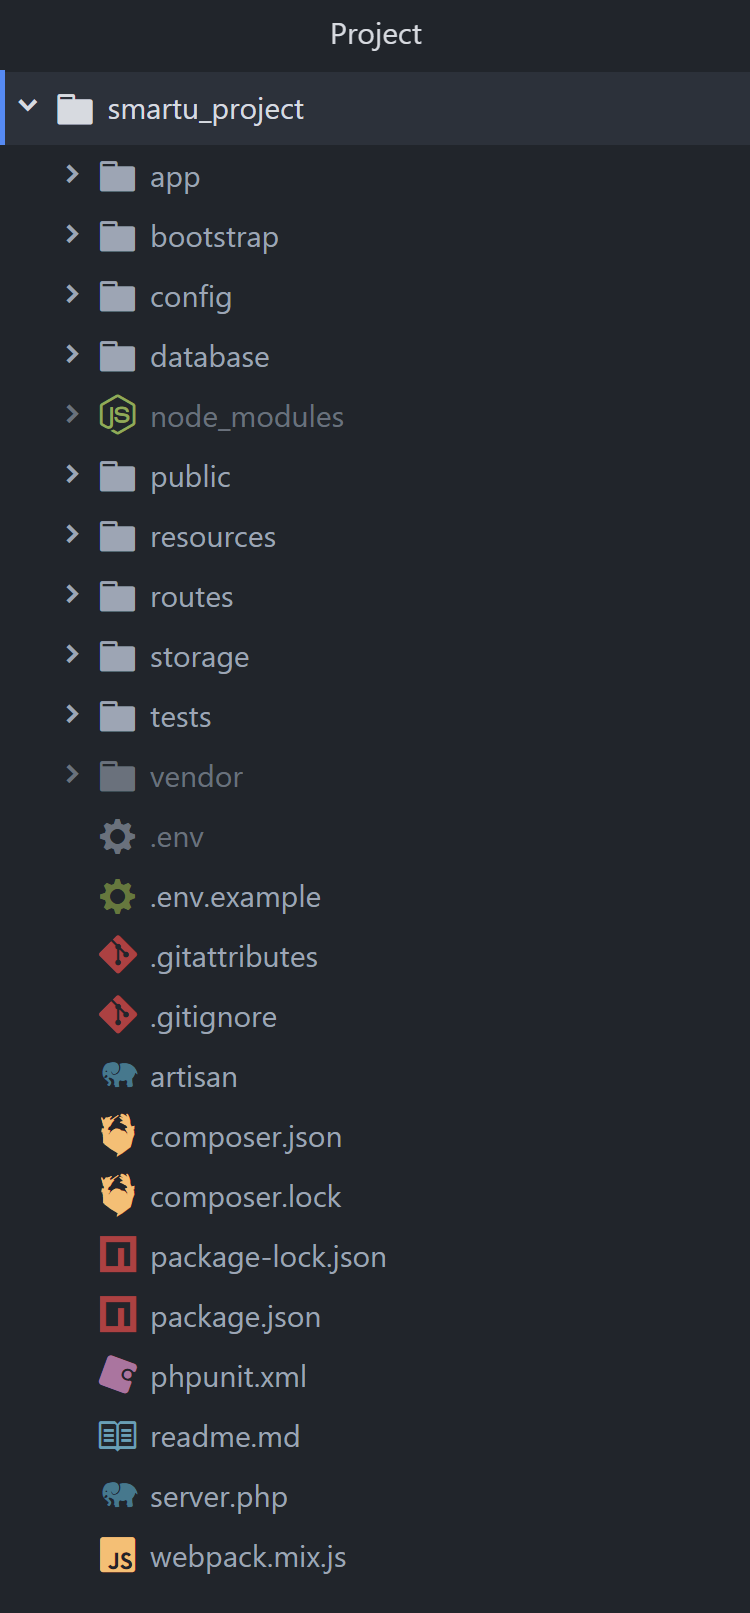
\includegraphics[scale=1.25]{directorios}
    \caption{Estructura de carpetas y ficheros del proyecto}
    \label{directorios}
\end{figure}

\subsection{Middlewares}
Laravel hace un extenso uso de los \textit{Middlewares}. Podemos definirlos como software intermediario que proporciona una capa de abstracción entre una aplicación y otra. En el caso de Laravel, nos proporciona por defecto una serie de middlewares que realizan varias tareas sin que nosotros tengamos que intervenir en ellas, liberando al programador de carga de trabajo.\\

Uno de los principales middleware que proporciona este framework es el de autenticación. Permite, por ejemplo, que un usuario autentificado en el sistema pueda realizar ciertas tareas y evita que aquellos que no lo están las puedan hacer, en cuyo caso los redigire a otra dirección que si tengan permitida. Otro middleware importante es el de la verificación del token CSRF, pero esto lo hablaremos con más detalle en el apartado de seguridad.

\subsubsection{Middleware de localización}
Con el objetivo de lograr que la aplicación web tuviera soporte \textbf{multilenguaje}, se ha hecho uso de un middleware personalizado que captura los parámetros de la URL y detecta si existe un código de idioma correcto, y en caso de no tenerlo, le añade el del idioma por defecto de la aplicación. Como se puede comprobar, los middlewares nos permiten delegar ciertas tareas para no tener que preocuparnos de nada y poder continuar el desarrollo.

\subsection{Patrones de diseño}
El uso de patrones de diseño es muy recomendable a la hora de desarrollar software. Laravel, por su funcionamiento interno, logra aplicar el patrón MVC mencionado anteriormente, pero no es el único que encontramos. Existen más patrones de diseño que se aplican para determinadas características, como por ejemplo:

\begin{description}
    \item [Builder] El patrón Builder permite separar la creación de un objeto complejo de su representación, con el fin de que el mismo proceso de construcción pueda usarse para crear diferentes representaciones. En Laravel podemos tomar como ejemplo la clase \textit{AuthManager}, que hereda de \textit{Manager}, siendo esta última la clase Builder que se encarga de construir los componentes seguros necesarios para almacenar informaciónde autentificación, ya sea en una variable de sesión o en una cookie.
    \item [Factoría] Este patrón permite definir una interfaz común de creación de objetos, pero deja a las subclases que sean ellas las que decidan qué objeto es el que quieren instanciar. Laravel hace un extenso uso de este patrón, por ejemplo, a la hora de crear conjuntos de reglas de validación de datos (usados habitualmente para comprobar los que se reciben a través de un formulario).
    \item [Estrategia] El patrón Estrategia o también conocido como \textit{Policy}, define una familia de algoritmos y los encapsula cada uno, haciendo que estos puedan ser reutilizados en cualquier momento.
    \item [Fachada] El patrón Fachada proporciona una interfaz unificada a un conjunto de interfaces de un subsistema. La fachada define una interfaz de alto nivel que hace que el subsistema sea más sencillo de usar. Laravel está construido con el uso de este patrón en casi todas partes, agrupando funcionalidades complejas en unas más simples de usar.
\end{description}

\section{Pruebas}
Para realizar la fase de pruebas de este proyecto, se ha seguido el proceso habitual de una \textbf{metodología ágil}, es decir, probar que las funcionalidades de la aplicación web funcionan correctamente en todos los posibles casos de uso. En concreto, se ha seguido el siguiente proceso:

\begin{itemize}
    \item El desarrollo se ha realizado implementando en primer lugar las \textbf{funcionalidades \textit{core}} o ensenciales de la aplicación, es decir, la gestión de los usuarios y los proyectos, así como la gestión de los diferentes idiomas que pueda haber disponibles.\\
    Se ha garantizado mediante pruebas que en este punto es posible crear usuarios y proyectos, y los usuarios invitados (no registrados) sólo pueden hacer operaciones de consulta.\\
    También se ha garantizado que el cambio de idioma de la aplicación se hace correctamente.
    \item Tras la funcionalidad esencial, se han implementado las \textbf{pequeñas funcionalidades} que no presentan un fuerte acoplamiento con otras y que, por ende, no dependen del funcionamiento de éstas, de modo que se puede garantizar más rápidamente su correcto funcionamiento.\\
    Entre las funcionalidades que se consideran ``auto-contenidas'' encontramos los comentarios de un proyecto, los avances, los ``Buena Idea'', las áreas y las especialidades.
    \item Por último, una vez que se ha realizado todo lo necesario para probar la funcionalidad esencial y las pequeñas funcionalidades auto-contenidas, se procedió a la implementación de las \textbf{funcionalidades más complejas} que requerían de la interacción entre otros componentes de la aplicación. Cada funcionalidad se iba probando en todos los posibles casos de uso.\\
    Aquí se incluye toda la funcionalidad relativa a las vacantes y las solicitudes para incorporarse como integrantes de un proyecto, y las notificaciones.
\end{itemize}

Debido a los problemas de tiempo que he tenido para realizar este proyecto, no he podido realizar pruebas más exahustivas de la implementación, o incluso pruebas unitarias. Para futuras ampliaciones de este proyecto (ya que se espera una continuación del mismo), sería apropiado realizar una colección de pruebas que se pudieran ejecutar de forma automatizada antes de proceder a incrementar el conjunto de funcionalidades de la aplicación web.

\section{Herramientas de desarrollo}
Para el desarrollo de este proyecto he utilizado el siguiente conjunto de herramientas y programas de desarrollo:

\begin{itemize}
    \item Laravel 5.5 con la versión 7 del lenguaje PHP.
    \item Servidor de pruebas XAMPP con instalación de Apache y MariaDB.
    \item Editor de texto Atom 1.19.
    \item Draw.io (diagramas del proyecto).
    \item Windows 10 Pro Versión 1703.
\end{itemize}

El proyecto es fácilmente portable a otros entornos de desarrollo siguiendo las instrucciones del anexo de intalación incluido en esta documentación.

% \chapter{Descripción de la aplicación web SmartU}

\chapter{Conclusiones y mejoras para el futuro}

\chapter{Anexos}
\label{ch:anexos}

\section{Ideas recopiladas de la sesión de \textit{Design Thinking}}
\label{sec:designthinking}
\begin{itemize}
    \item \textbf{Aspectos positivos}
    \begin{itemize}
        \item Pensar y actuar, comprometerme.
        \item ¡Armarse de valor! Empezar y luego ir mejorando aspectos, uno por uno.
        \item Sienten que la universidad no fomenta el trabajo en equipo cuando es algo que las empresas demandan (se ve como algo positivo a aprovechar).
        \item Oigo que las empresas siempre están buscando talentos y gente con ideas para ayudarles a llevarlas a cabo.
        \item Puede dar difusión a una buena idea.
        \item El TFG de mi carrera es muy aburrido (visto como oportunidad).
        \item Veo posibilidades de mejorar la realidad física a través de la realidad virtual. Pensar.
        \item Es una oportunidad de crear proyectos interesantes y experiencias.
        \item Proponer herramientas online y virtuales y generar documentación.
        \item Múltiples posibilidades. Inquietud.
        \item Trabajar duro para llegar a la cohesión. Investigar acerca de todo, el máximo posible. Afrontar el proyecto sin temor al fracaso.
        \item Frustración por no desarrollar una idea propia.
        \item Apostar por ideas innovadoras de TFG. Buscar ideas/productos interesantes para motivar.
        \item Veo un gran distanciamiento entre los distintos campus y no saben lo que pasa entre unos y otros.
    \end{itemize}
    \item \textbf{Ideas}
    \begin{itemize}
        \item Identidad visual.
        \item Comunicación.
        \item Plataforma web.
        \item Jornadas de estudiantes como forma de conocer sus necesidades e incertidumbres.
        \item Fomentar espacios virtuales para comunicación, reuniones y conocimiento.
        \item Fomentar espacios físicos de debate y trabajo (ámbito lúdico, forma de llegar a la sociedad).
    \end{itemize}
    \item \textbf{Objetivos}
    \begin{itemize}
        \item Mapa geográfico de proyectos que permitan acceder al proyecto.
        \item Proyectos conectados entre sí, por tipo.
        \item Hay que crear grupos muy comprometidos y concienciados.
        \item Dificultades, reuniones
        \item Posibilidad de llegar a todos.
        \item Exposición en público.
        \item Crear congresos y seminarios sobre el proyecto interdisciplinar.
        \item Síntesis de ideas para transformarlas en contenido a exponer en redes y otros medios y así dar repercusión al proyecto.
    \end{itemize}
    \item \textbf{Limitaciones}
    \begin{itemize}
        \item No se conoce. Dudas acerca de la viabilidad. No lo entienden. Les atrae como para crear una empresa.
        \item Cómo dar más difusión a los trabajos TFG.
        \item Huimos del tema por miedo a suspender. Vamos a lo fácil para sacar la carrera y no nos complicamos.
        \item Oigo que la gente tiene buenas ideas que le gustaría desarrollar, pero les falta gente que sepa de ciertas cosas.
        \item Cuesta trabajo encontrar tiempo para dedicárselo.
        \item No hay espacios para trabajar en grupo. No hay espacio ni tiempo suficiente para trabajar.
        \item Es un mayor esfuerzo de lo que parece habitual.
        \item No hay tiempo y faltan espacios.
        \item Grandes ideas, propuestas interesantes. Pero hay limitaciones de tiempo y material.
        \item Inseguridad. Ilusión por realizar algo innovador. Falta de un anteproyecto que una las diferentes ramas.
        \item Hay que conformarse con el TFG establecido.
        \item Oigo a la gente quejarse de que trabajar en equipo a veces no sale bien.
        \item No hay tiempo para reuniones y organizar.
        \item Exceso de trámites para realizar un TFG.
        \item Piensan que trabajar en equipo es un engorro y que siempre sale mal.
        \item No existen herramientas para hacer diferentes TFG.
        \item Falta de ayuda por parte de la universidad y el ayuntamiento.
        \item Como ven que es difícil trabajar en equipo, lo que hacen es conformarse con un proyecto más simple que les gusta menos.
        \item Con desesperación, con esperanza, con oportunidades.
        \item Necesidad de implicación (nosotros mismos, menos integrantes). Necesidad de sintetizar las ideas. Si una persona no conoce el proyecto, o quiere participar, una idea clara.
        \item Plazos y forma de organización a veces muy rígida.
        \item Veo que la gente no está motivada a trabajar en equipo y prefieren trabajar solos.
        \item Incertidumbre, amparo, curiosidad.
        \item Inestabilidad, falta de conexión.
    \end{itemize}
\end{itemize}

\section{Actas de reunión del equipo}
\label{sec:actas}
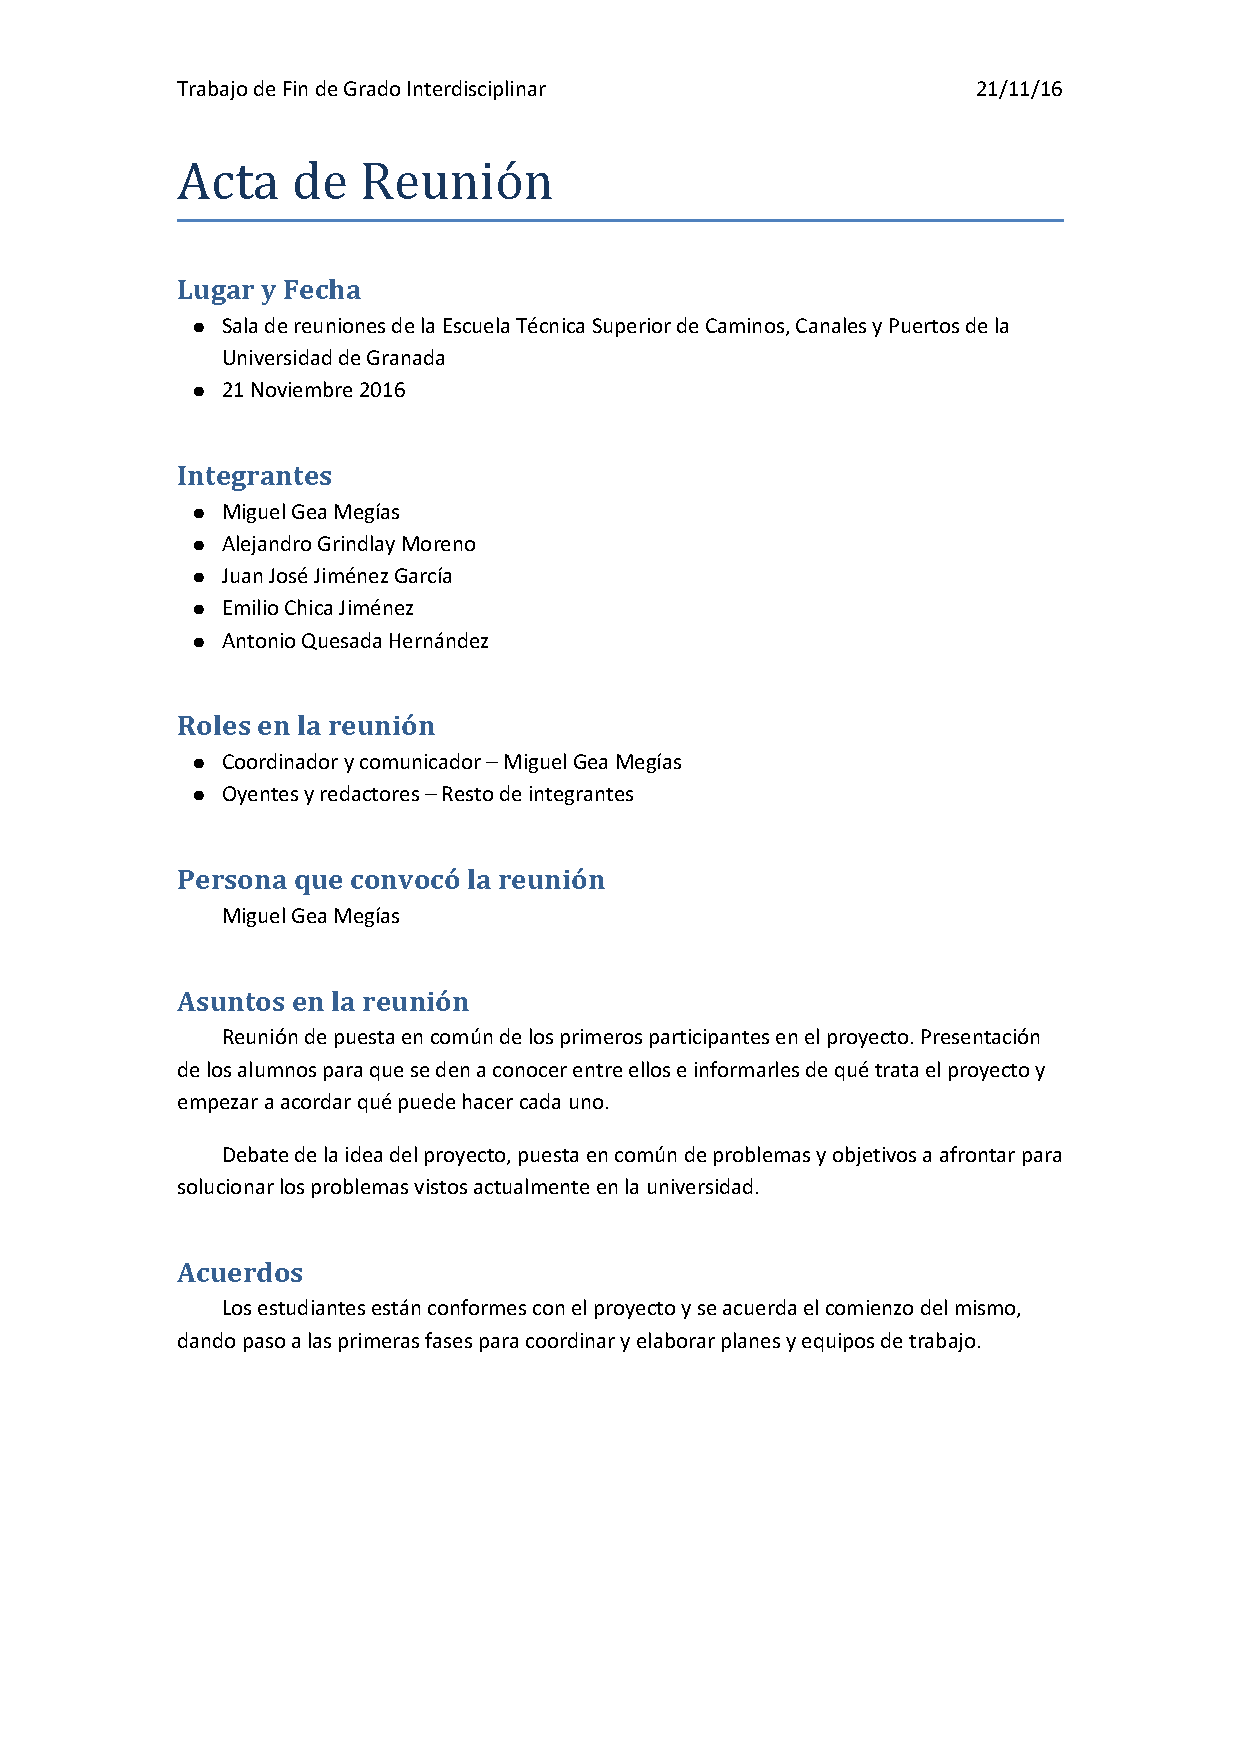
\includepdf[pages=1-]{meetings/01.pdf}
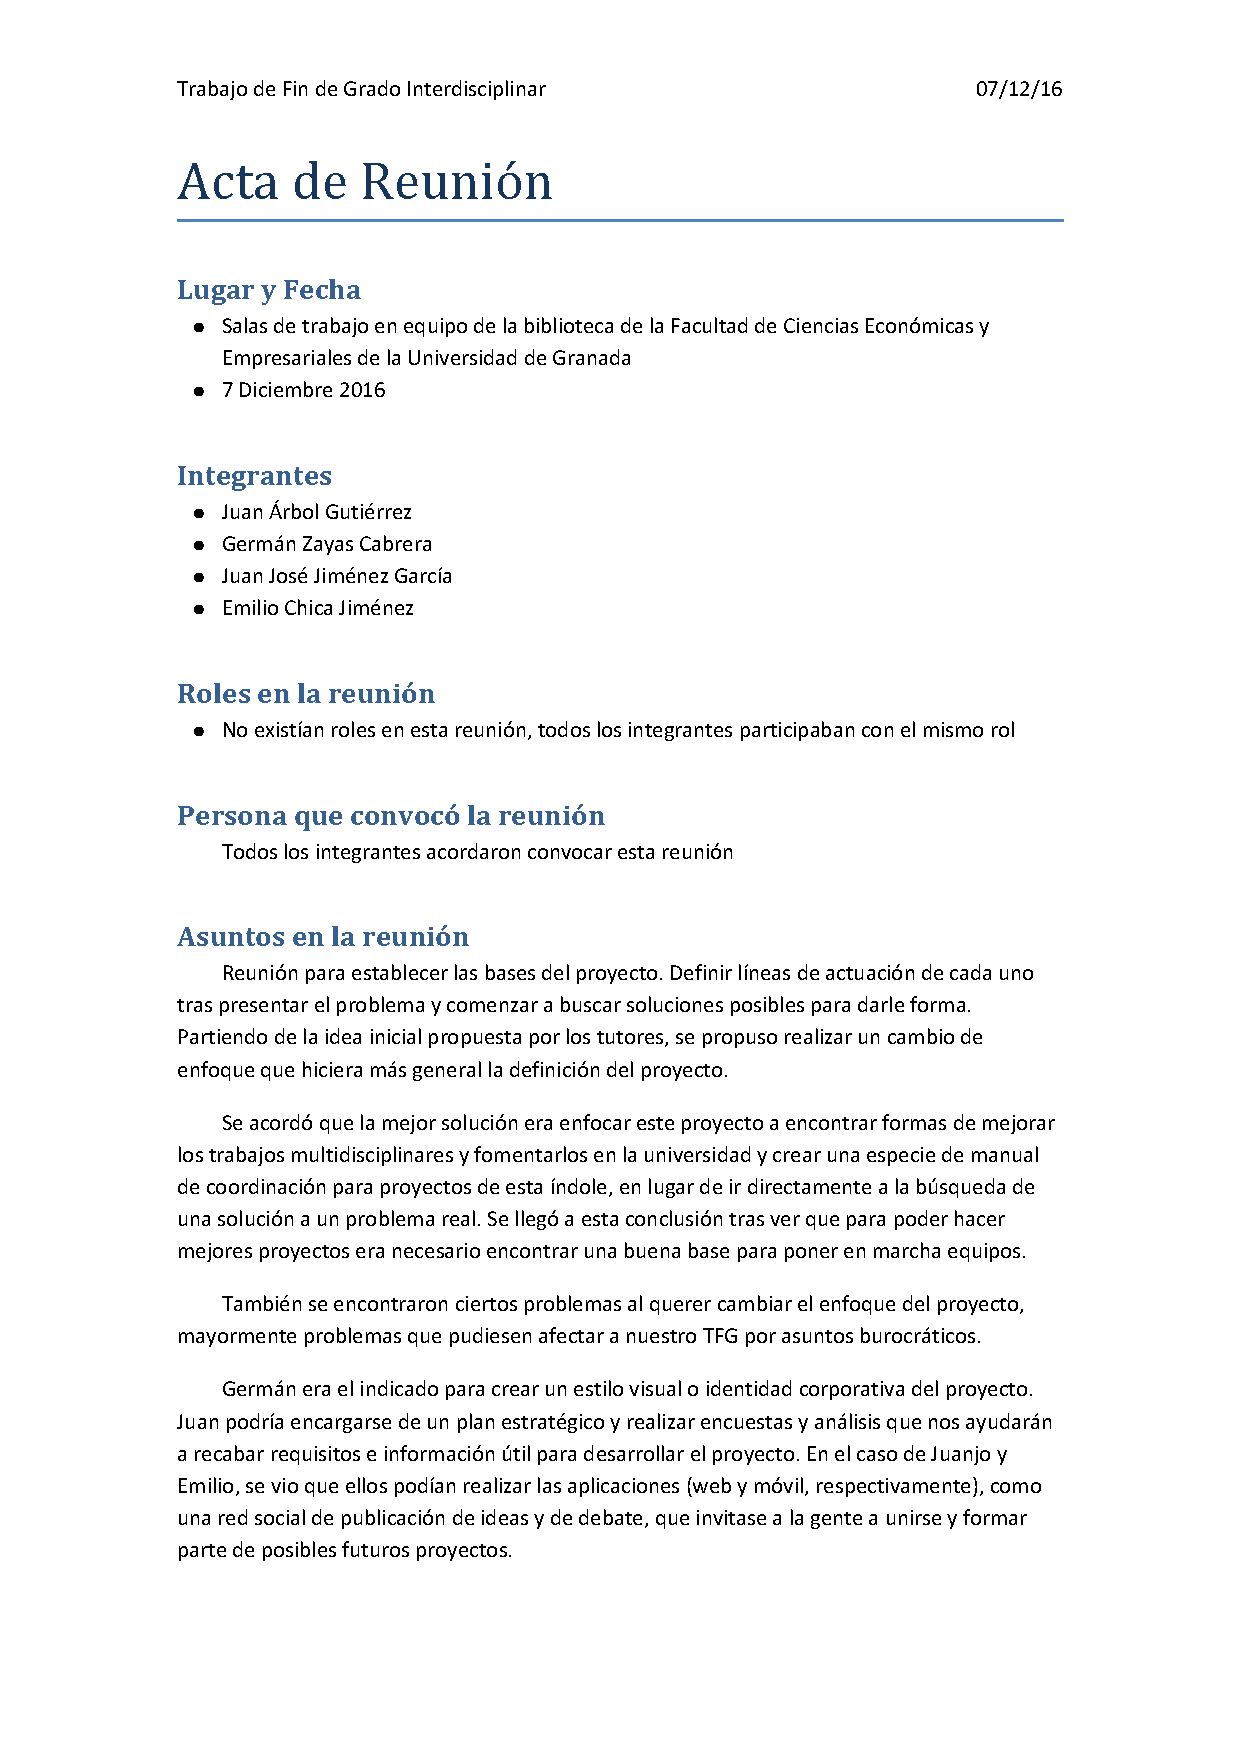
\includepdf[pages=1-]{meetings/02.pdf}
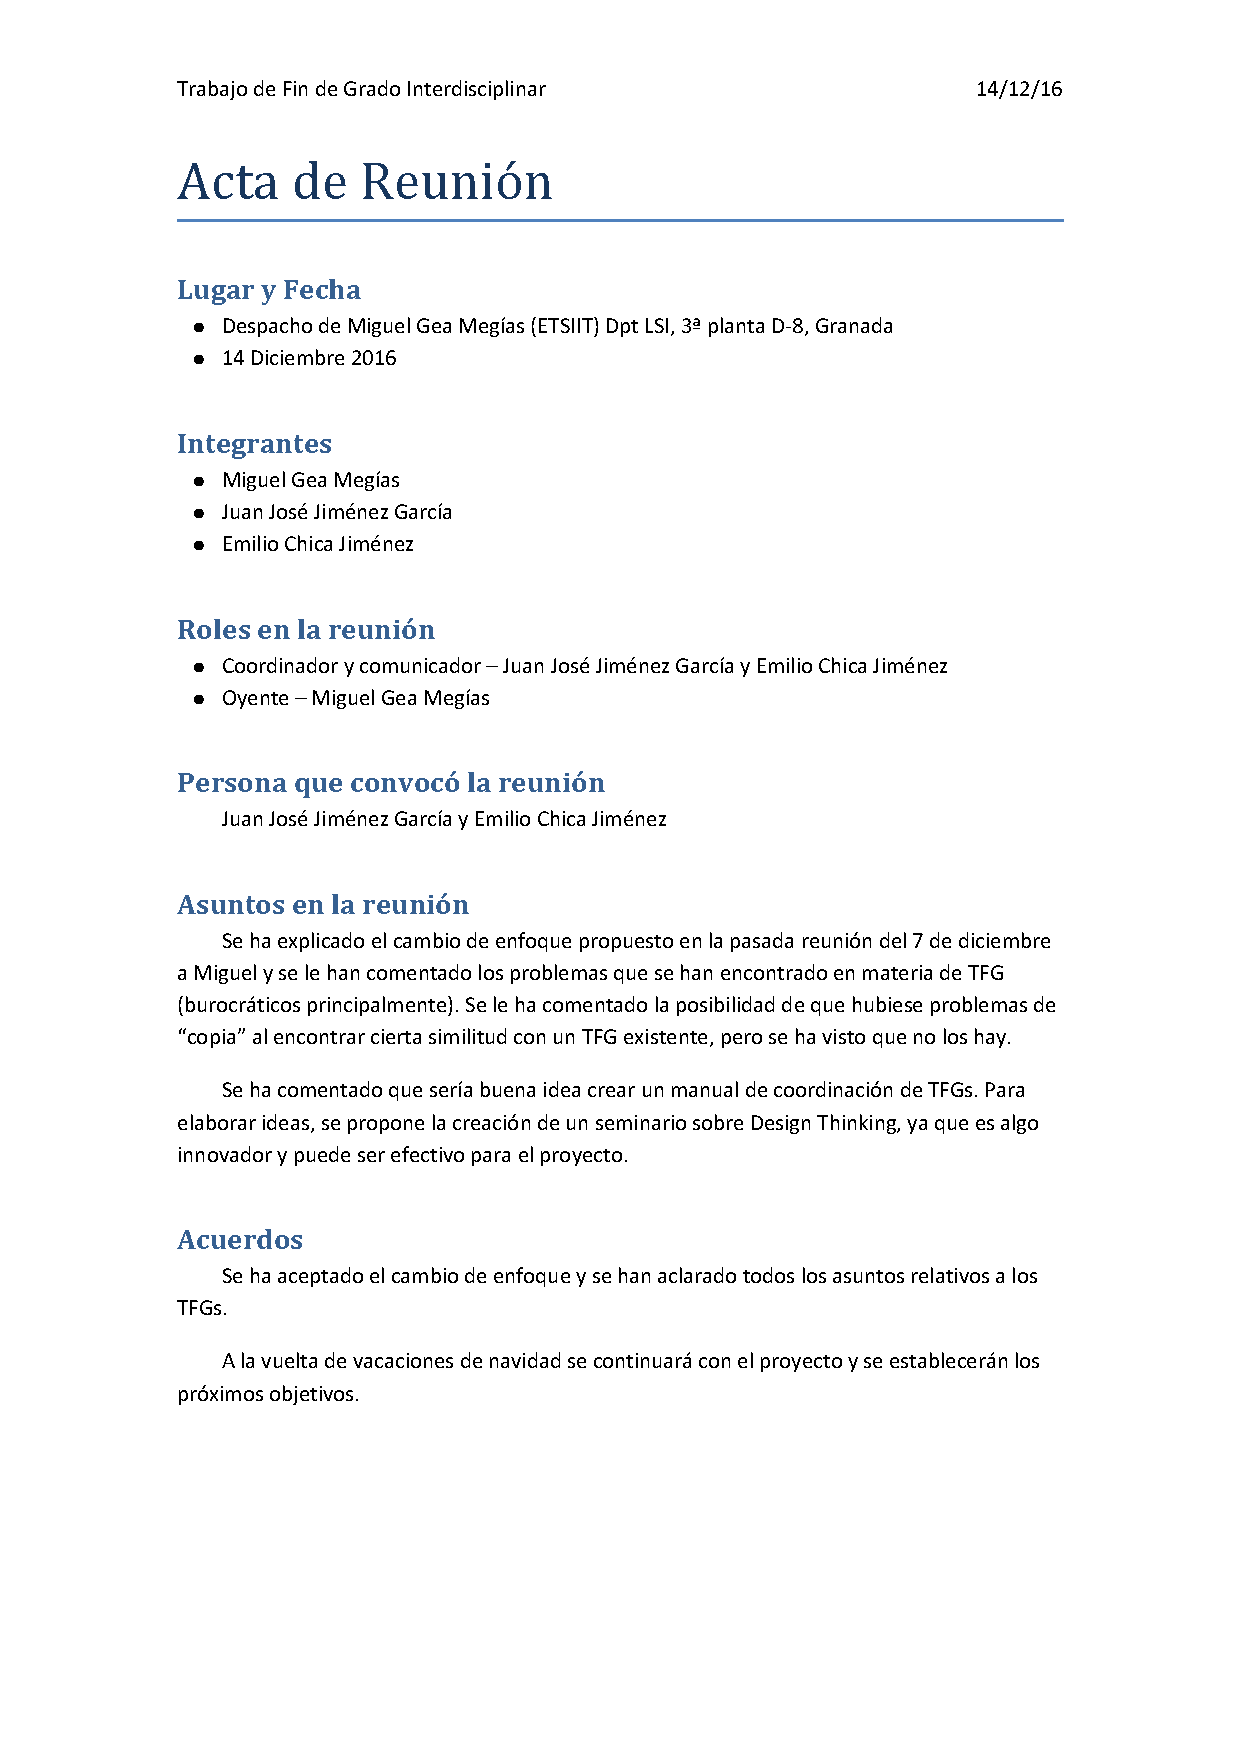
\includepdf[pages=1-]{meetings/03.pdf}
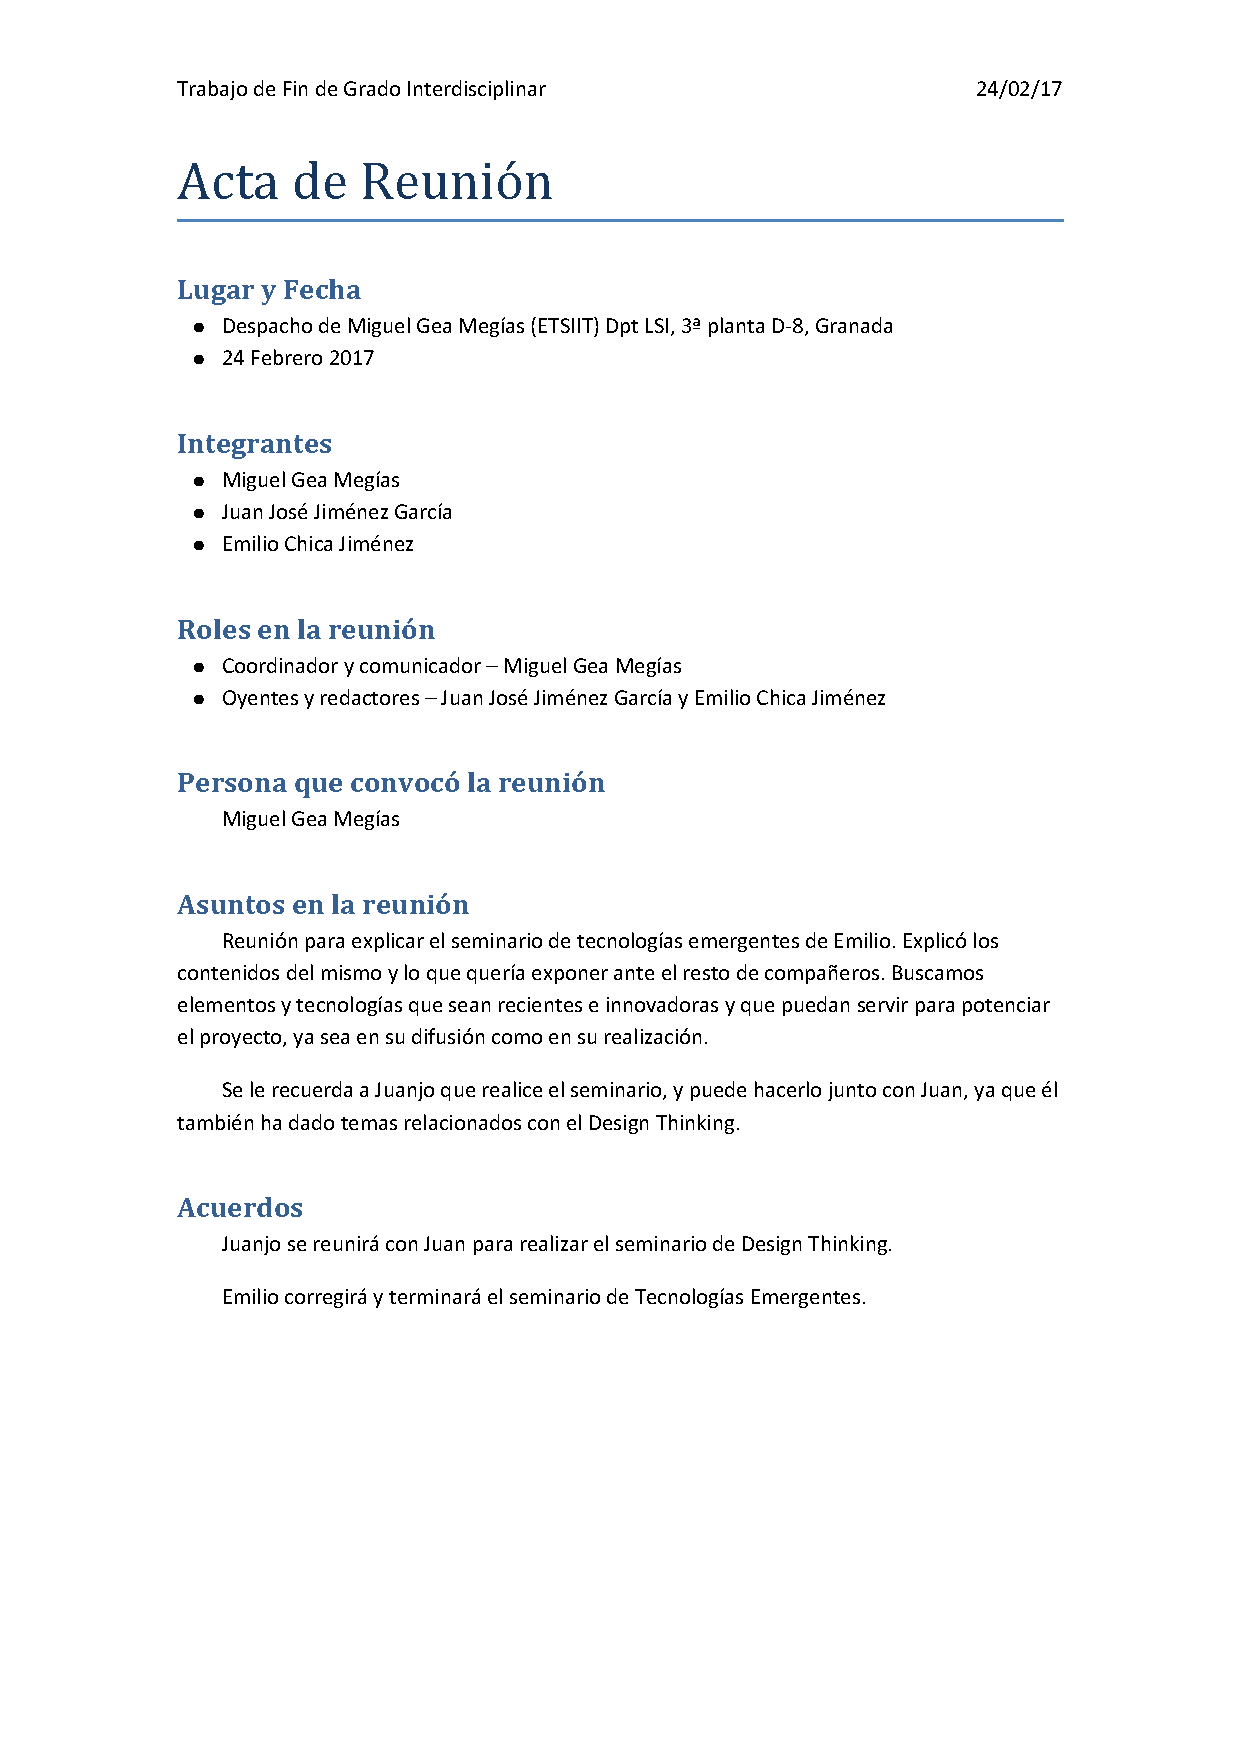
\includepdf[pages=1-]{meetings/04.pdf}
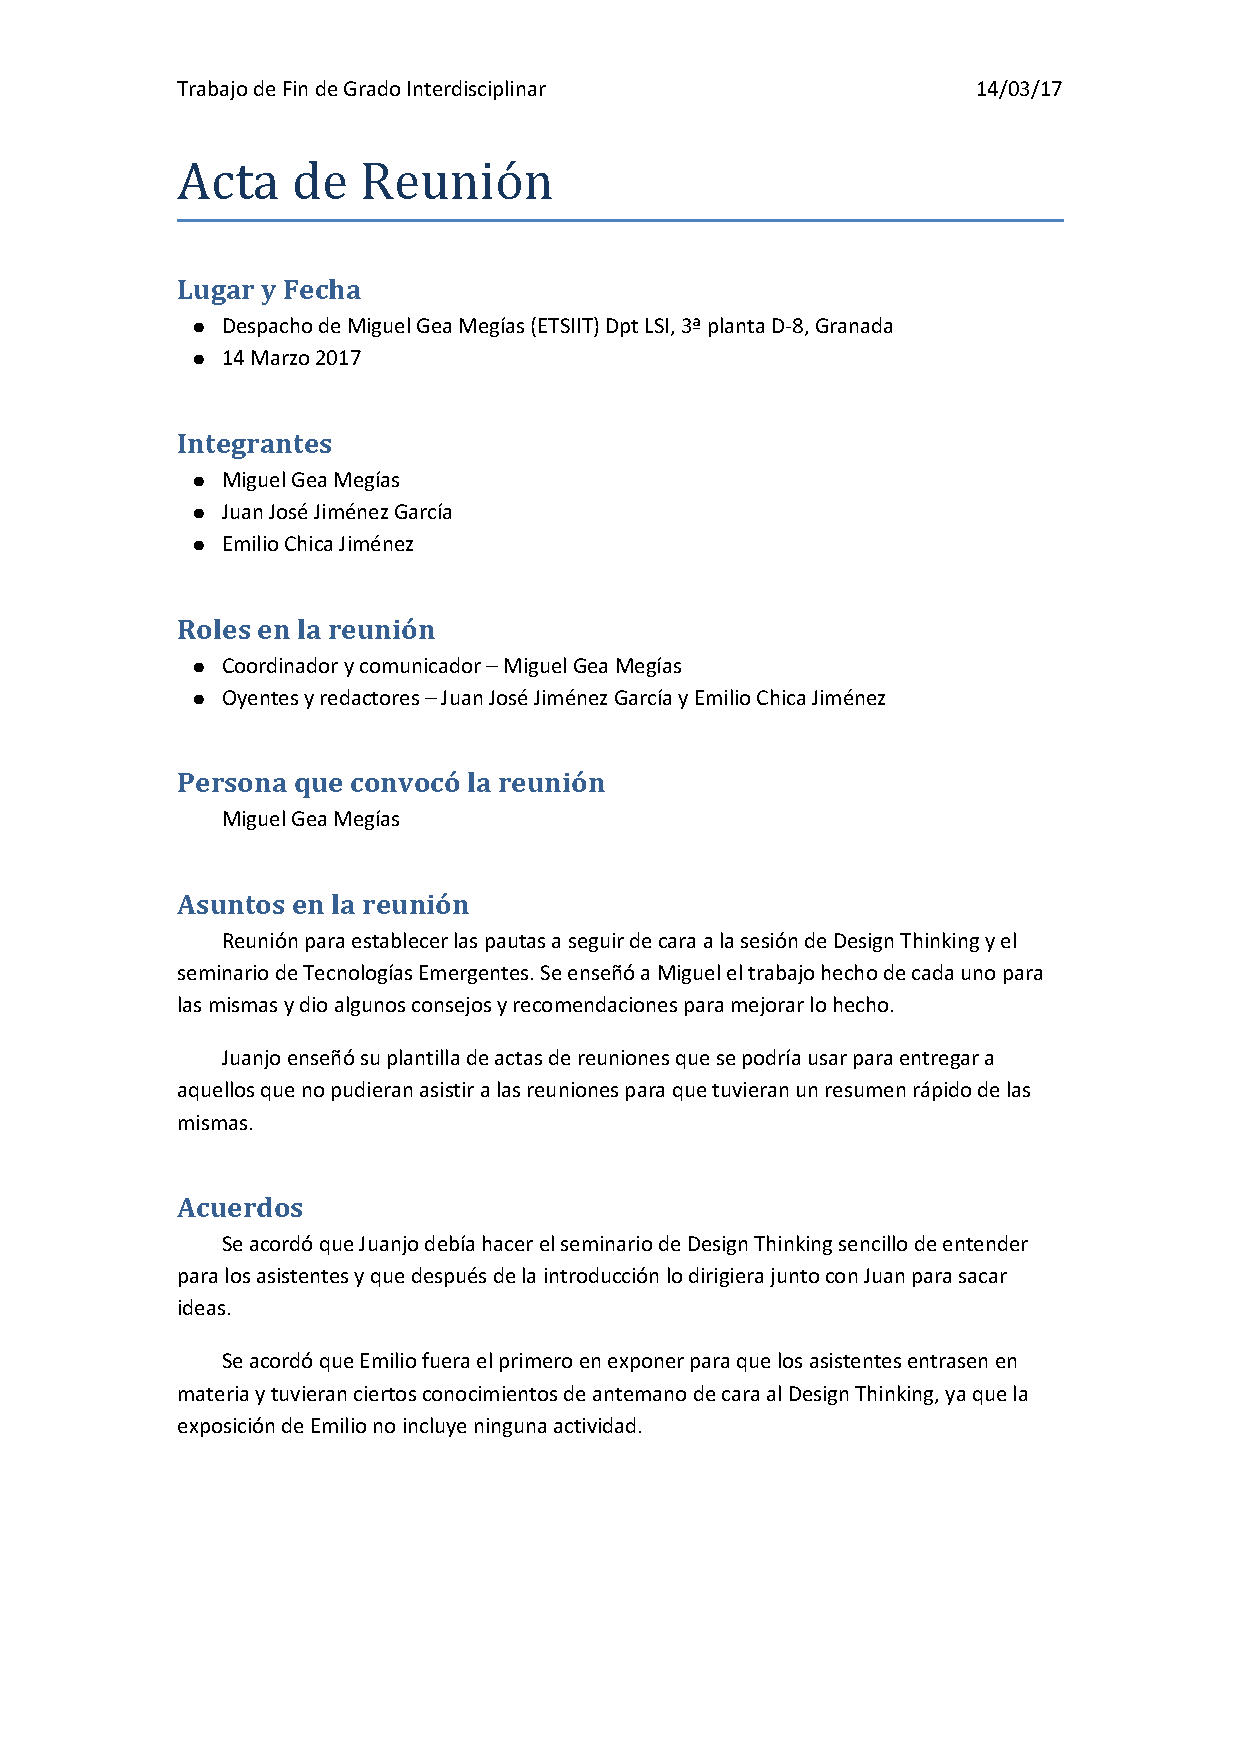
\includepdf[pages=1-]{meetings/05.pdf}
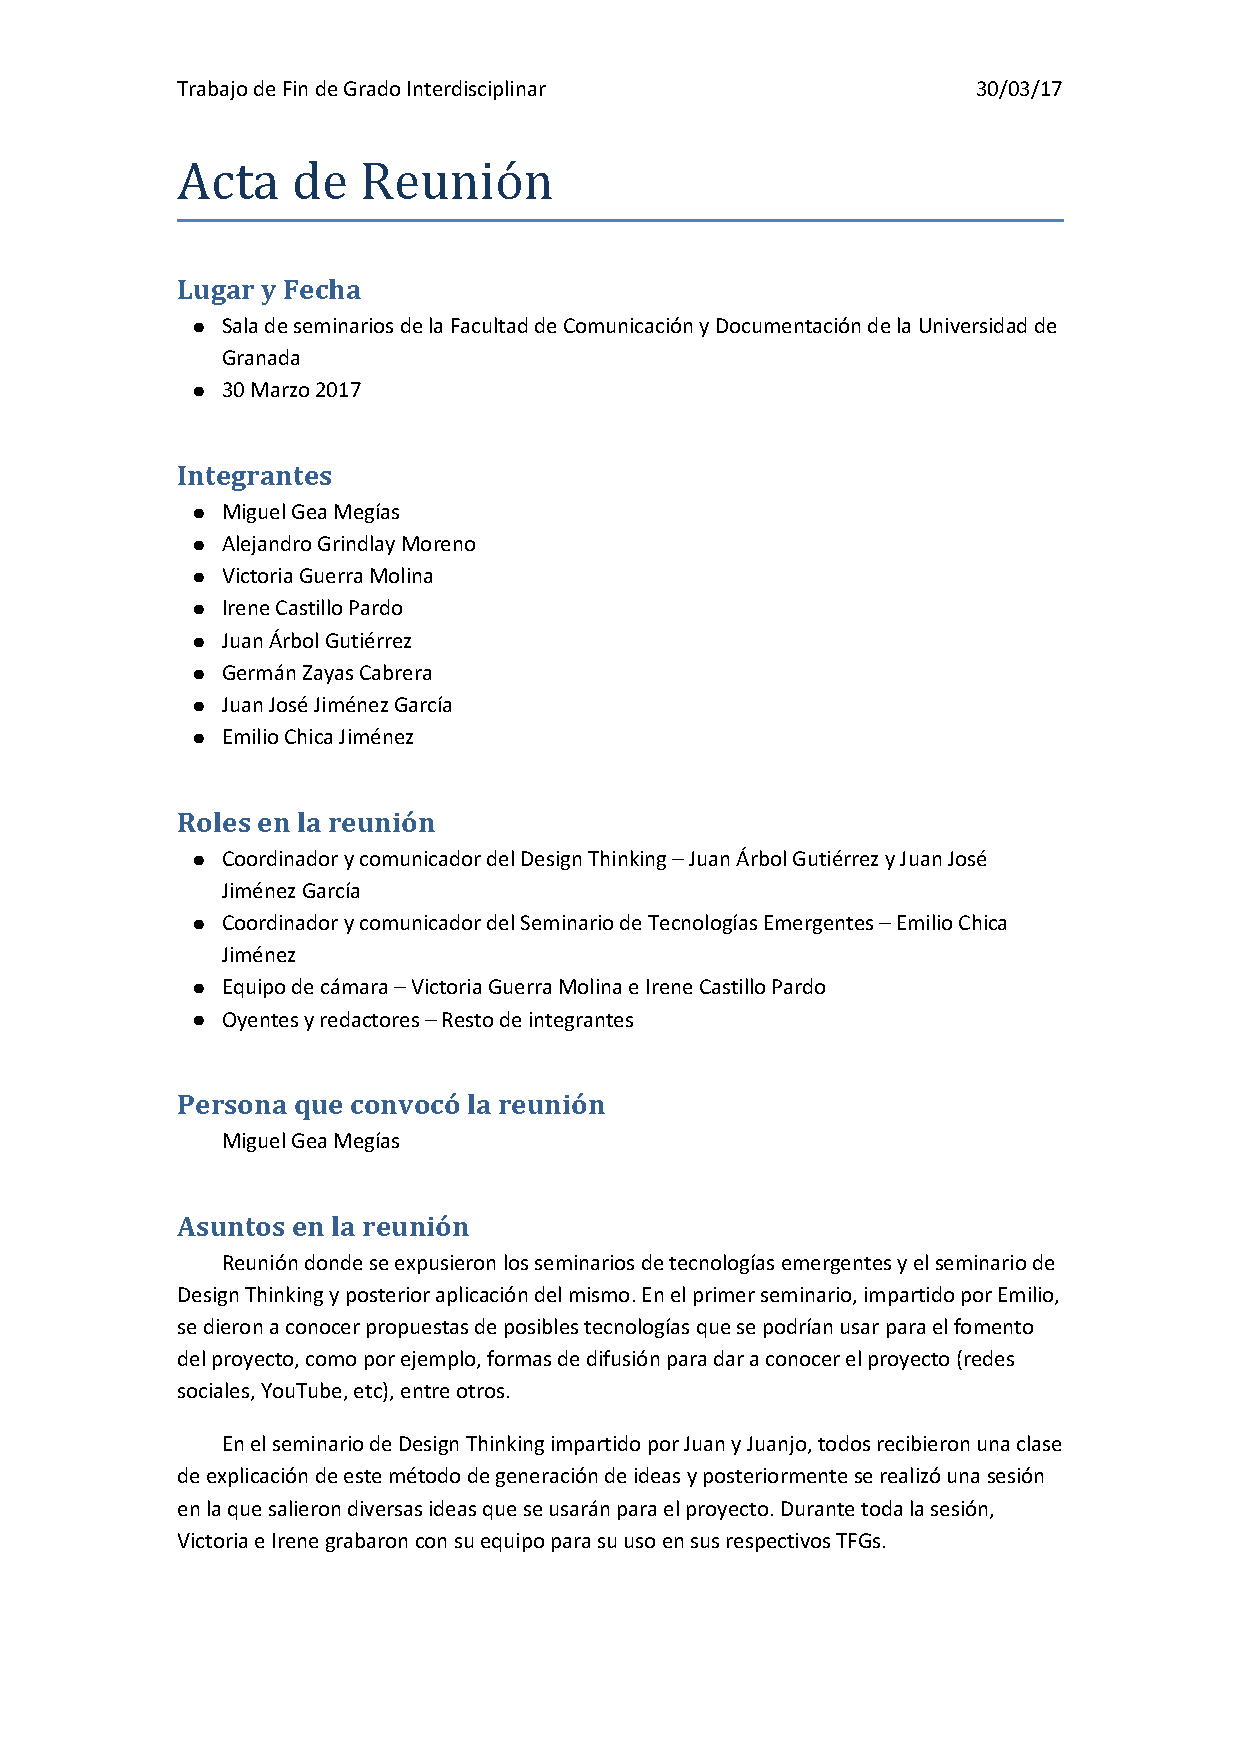
\includepdf[pages=1-]{meetings/06.pdf}
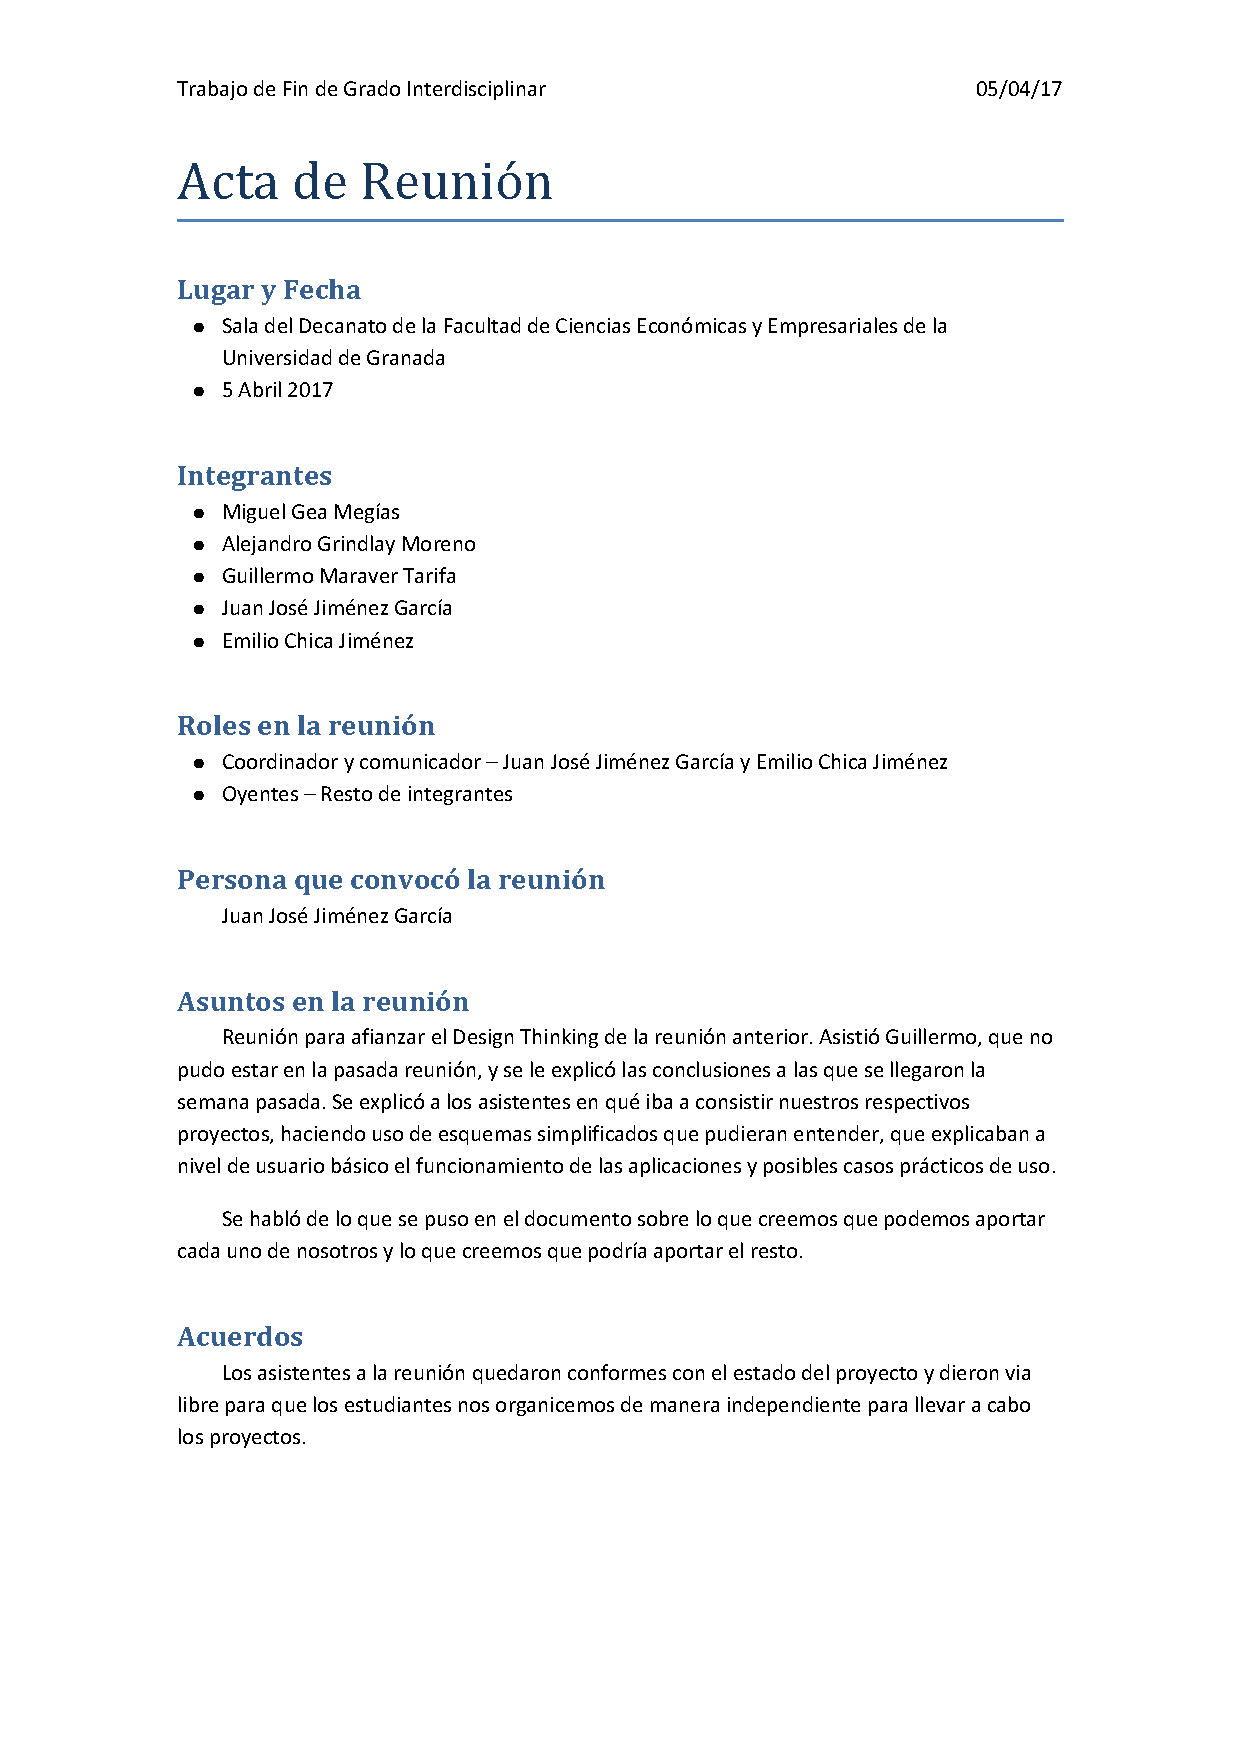
\includepdf[pages=1-]{meetings/07.pdf}
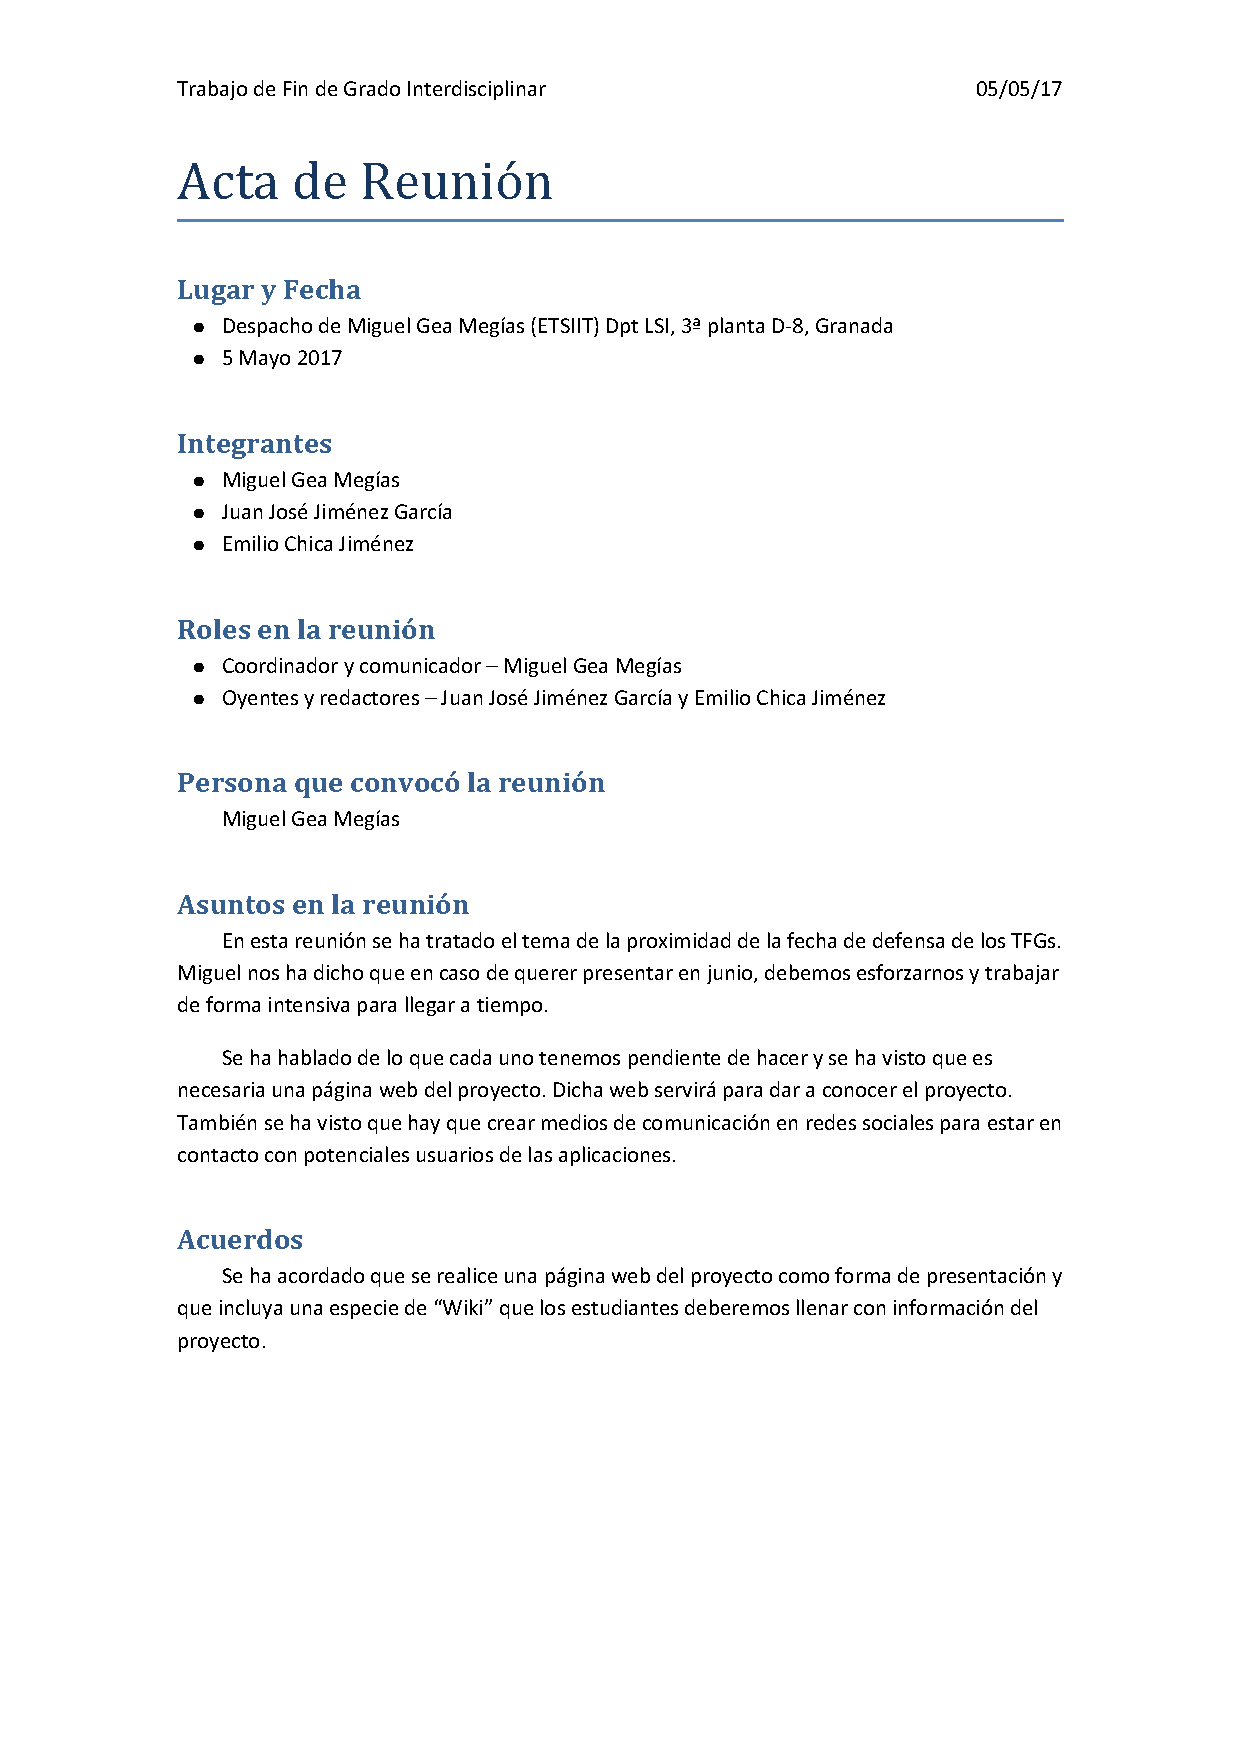
\includepdf[pages=1-]{meetings/08.pdf}
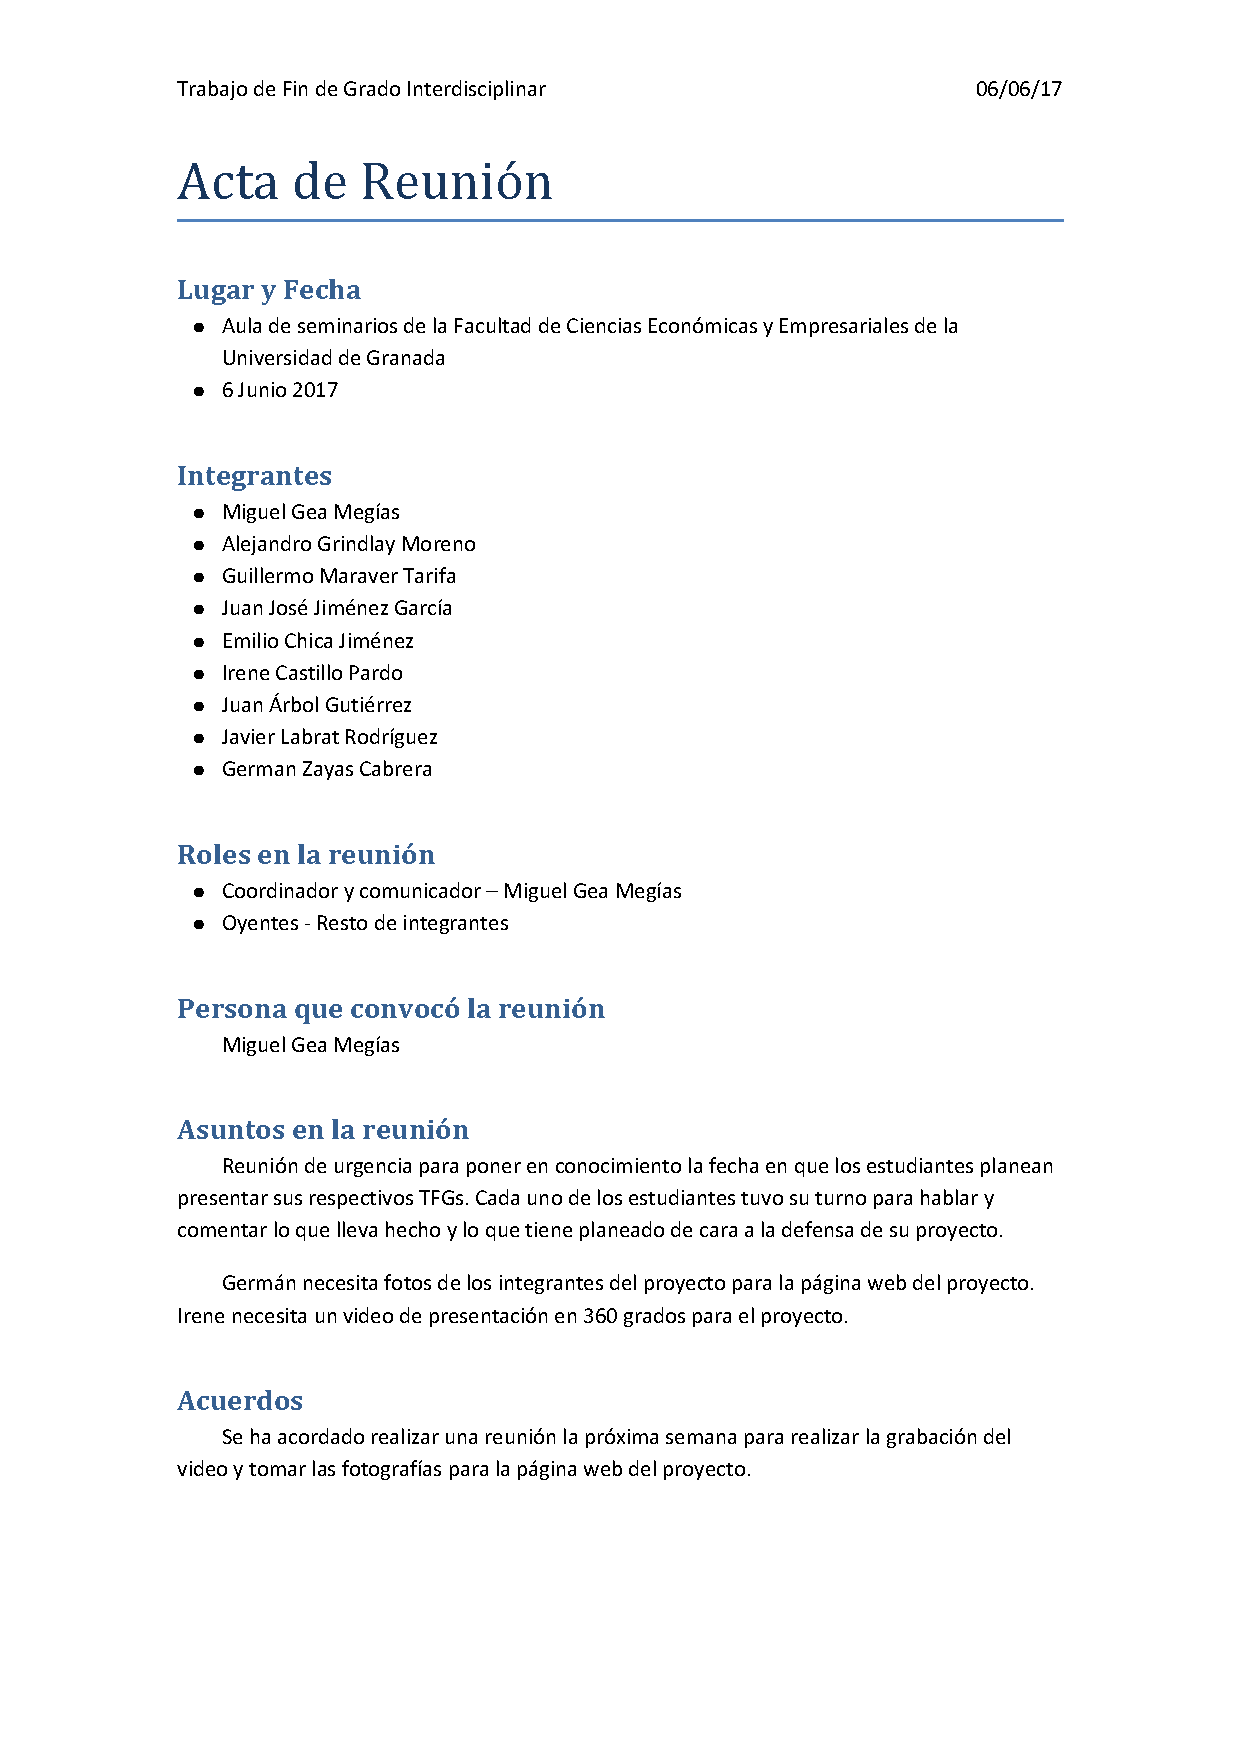
\includepdf[pages=1-]{meetings/09.pdf}
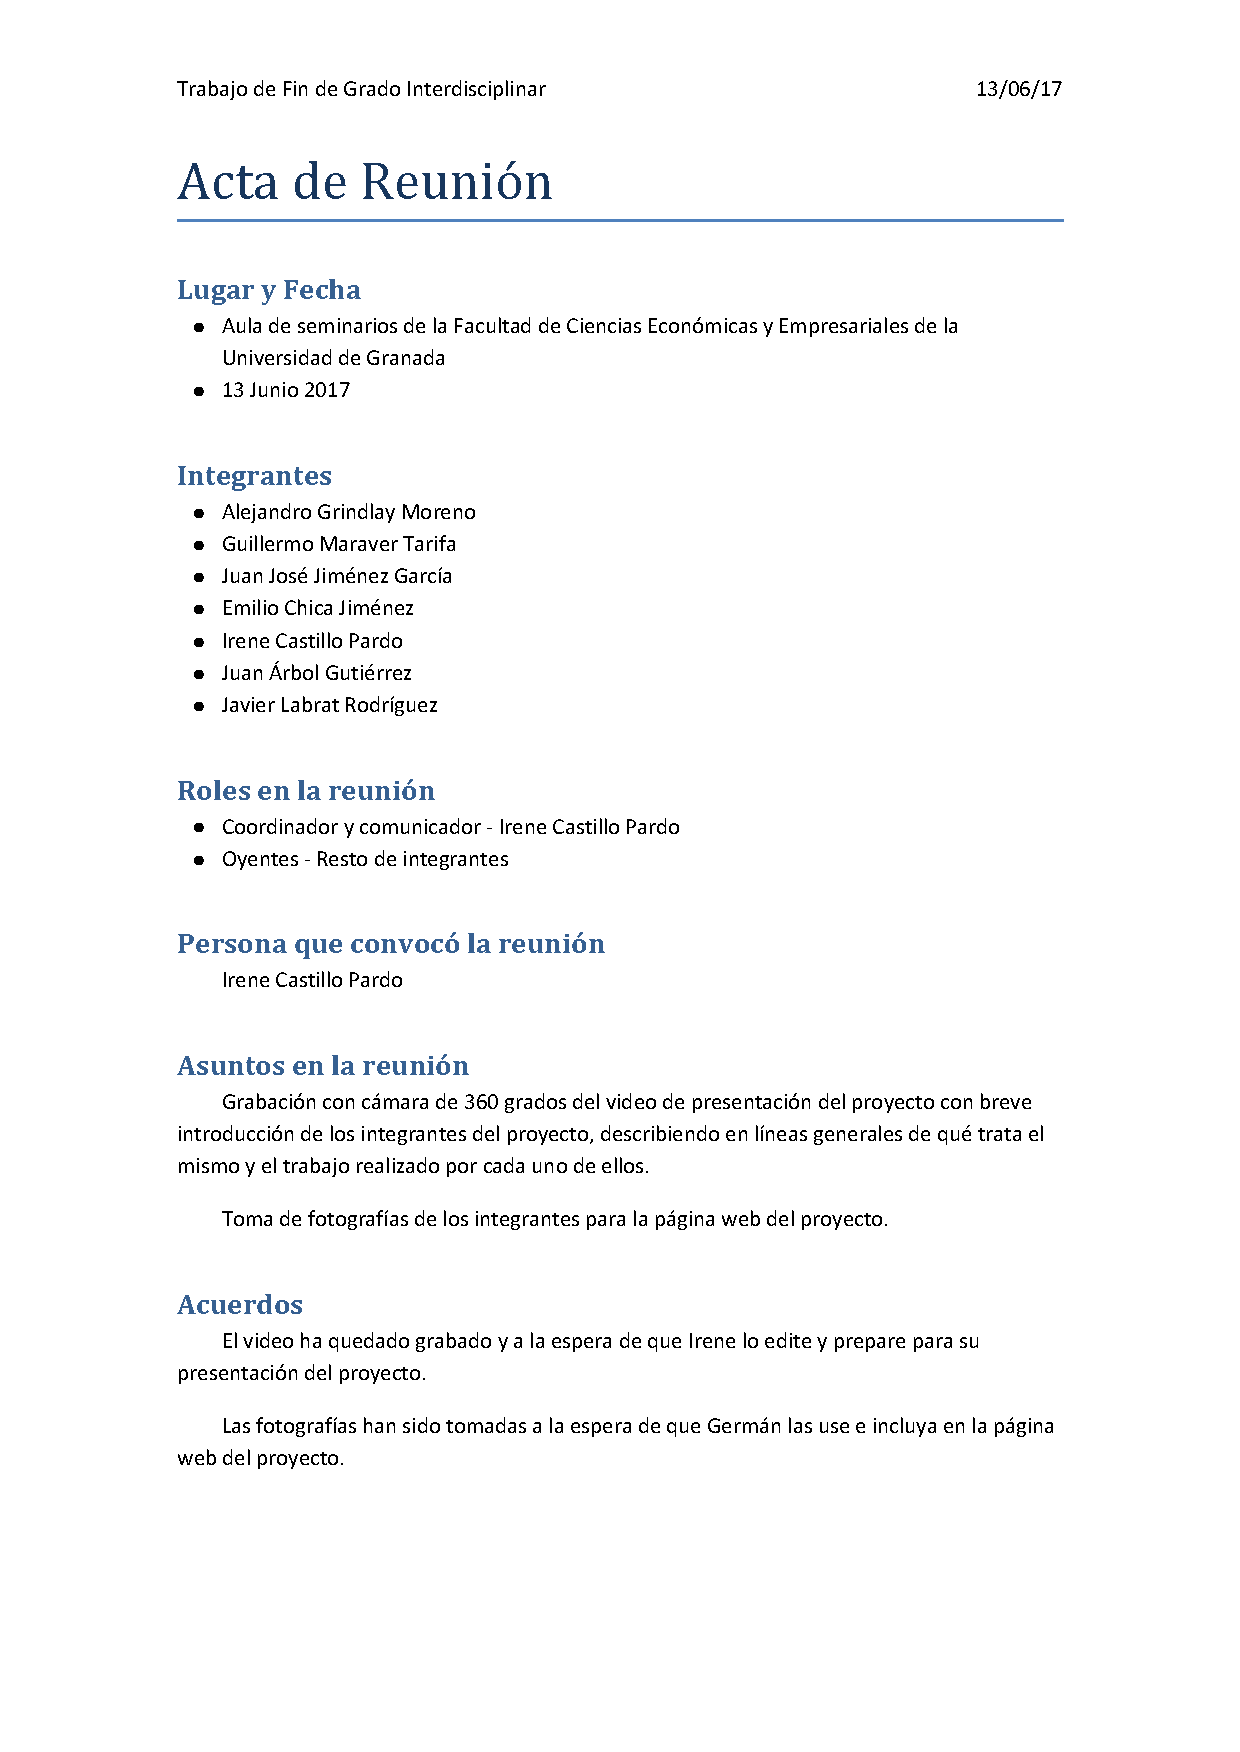
\includepdf[pages=1-]{meetings/10.pdf}


% Glosario de términos
\backmatter
\begingroup
	\setlength\parindent{0pt}
	\chapter{Glosario de términos}

\begin{description}
    \item[Equipo multidisciplinar] Conjunto de personas, con diferentes formaciones académicas y experiencias profesionales, que operan en conjunto, durante un tiempo determinado, abocados a resolver un problema complejo, es decir, que tienen un objetivo común. Cada individuo es consciente de su papel y del papel de los demás, y trabajan en conjunto bajo la dirección de un coordinador.
    \item[StartUp] Empresa emergente que busca arrancar, emprender o montar un negocio, generalmente apoyada en la tecnología para su desarrollo. Son ideas que innovan el mercado y buscan facilitar los procesos complicados, enfocadas a diferentes temas y usos. Generalmente son empresas asociadas a la innovación, al desarrollo de tecnologías, al diseño web o al desarrollo web.
    \item[Sinergia] La sinergia es una propiedad inherente de los sistemas que establece que las interacciones entre las partes o componentes de un sistema generan un valor agregado mayor al que se lograría si cada componente funcionara por separado.\\
    Aplicado al trabajo en equipo, surgen sinergias cuando la colaboración entre miembros produce más resultados que haciéndo cada uno su parte sin contar con el otro.
    \item[Framework de desarrollo] Es una estructura conceptual y tecnológica de asistencia definida, normalmente, con artefactos o módulos concretos de software, que puede servir de base para la organización y desarrollo de software. Típicamente, puede incluir soporte de programas, bibliotecas, y un lenguaje interpretado, entre otras herramientas, para así ayudar a desarrollar y unir los diferentes componentes de un proyecto.
    \item[Diseño adaptable] El diseño adaptable establece que un sistema informático debe ser reactivo a la interacción del usuario con el mismo y al entorno en el que se encuentra. Esto quiere decir que ha de ``adaptarse'' a todo tipo de dispositivos donde se esté ejecutando o visualizando.
    \item[Diseño \textit{Mobile First}] es una filosofía de diseño que establece que todo desarrollo debe centrar su diseño en visualizar cómo se vería en un dispositivo móvil, y a partir de ese punto ampliar el tamaño de la pantalla e ir reorganizando los elementos.\\
    Por lo general, el diseño \textit{mobile first} comienza apilando uno encima de otro los elementos de la interfaz, y a medida que se gana espacio horizontal, colocar en este los elementos que estaban al fondo.
\end{description}

\endgroup

% Bibliografía
\newpage
\begin{thebibliography}{99}
	\addcontentsline{toc}{chapter}{Bibliografía}

\bibitem{globalizacion} {\tt Globalización - Wikipedia}\\
\url{https://es.wikipedia.org/wiki/Globalizaci%C3%B3n}

\bibitem{ugremprende} {\tt UGR Emprendedora - Página principal}\\
\url{https://ugremprendedora.ugr.es/}

\bibitem{h2020} {\tt Horizon 2020 - Página principal}\\
\url{https://ec.europa.eu/programmes/horizon2020/}

\bibitem{agilereport} {\tt Top 10 Insights from the 11th Annual State of Agile Report}\\
\url{https://explore.versionone.com/state-of-agile/top-10-insights-from-the-11th-annual-state-of-agile-report-2}

\bibitem{health1} {\tt PubMed Central - Multidisciplinary in-hospital teams improve patient outcomes: A review}\\
\url{https://www.ncbi.nlm.nih.gov/pmc/articles/PMC4173201/}

\bibitem{health2} {\tt PubMed Central - Benefits of multidisciplinary teamwork in the management of breast cancer}\\
\url{https://www.ncbi.nlm.nih.gov/pmc/articles/PMC3929250/}

\bibitem{neuroped} {\tt Imagen original de NeuroPed - Enlace}\\
\url{http://www.neuroped.es/equipo-multidisciplinar/}

\bibitem{medialabugr} {\tt Medialab UGR - Página principal}\\
\url{http://medialab.ugr.es/}

\bibitem{linkuma} {\tt Link by UMA-ATech (Universidad de Málaga) - Página principal}\\
\url{http://www.link.uma.es/}

\bibitem{linkedin} {\tt LinkedIn - Página principal}\\
\url{https://es.linkedin.com/}

\bibitem{kickstarter} {\tt Kickstarter - Página principal}\\
\url{https://www.kickstarter.com/}

\bibitem{contentwater} {\tt Imagen original de Wikimedia - Enlace}\\
\url{https://commons.wikimedia.org/wiki/File:Content_is_like_water.png}

\bibitem{bootstrap} {\tt Bootstrap Framework - Página principal}\\
\url{https://getbootstrap.com/}

\bibitem{framework} {\tt Framework - Wikipedia}\\
\url{https://es.wikipedia.org/wiki/Framework}

\bibitem{startup} {\tt Startup - Wikipedia}\\
\url{https://es.wikipedia.org/wiki/Empresa_emergente}

\bibitem{whatsapp} {\tt WhatsApp - Página oficial}\\
\url{https://www.whatsapp.com/}

\bibitem{slack} {\tt Slack - Página oficial}\\
\url{https://slack.com/}

\bibitem{googlecalendar} {\tt Google Calendar - Página oficial}\\
\url{https://www.google.com/calendar}

\bibitem{googledrive} {\tt Google Drive - Página oficial}\\
\url{https://www.google.com/drive}

\bibitem{laravel} {\tt Laravel - Documentación oficial}\\
\url{https://laravel.com/docs/5.5}

\bibitem{xampp} {\tt XAMPP - Página oficial}\\
\url{https://www.apachefriends.org/es/index.html}





















% \subsubsection*{Libros consultados durante la realización del proyecto:}
% \bibitem{stevekrug}
% Steve Krug.
% \newblock {\em Don't make me think! : a common sense approach to web usability.}
% \newblock New Riders, 2006.
% \newblock ISBN: 0321344758.
%
% \bibitem{jakonielsen}
% Jakob Nielsen.
% \newblock {\em 10 Usability Heuristics for User Interface Design.}
% \newblock Nielsen Norman Group, 1995.
%
% \bibitem{melenaalva}
% María Elena Alva Obeso.
% \newblock {\em Metodología de medición y evaluación de la usabilidad en sitios Web educativos.}
% \newblock Universidad de Oviedo, 2005.
% \newblock ISBN: 9788483175842.
%
% \bibitem{ericreiss}
% Eric Reiss.
% \newblock {\em Usable usability: simple steps for making stuff better .}
% \newblock John Wiley \& Sons, Inc., 2012.
% \newblock ISBN: 9781118185476.
%
% \subsubsection*{Artículos sobre las metodologías utilizadas en el proyecto:}
% \bibitem{art_14} `'The Distributed Course'. Stephen Downes. 2008. \url{https://sites.google.com/site/themoocguide/3-cck08---the-distributed-course}
%
% \bibitem{art_13} ``Top Universities Test the Online Appeal of Free''. Richard Pérez-Peña. 18/07/2012. \url{http://www.nytimes.com/2012/07/18/education/top-universities-test-the-online-appeal-of-free.html}
%
% \bibitem{art_12} `'Cuando un profesor de la Gran Depresión predijo la educación online'. Jonathan Préstamo. 09/06/2017. \url{http://www.teknoplof.com/2017/06/09/cuando-profesor-la-gran-depresion-predijo-la-educacion-online/}
%
% \bibitem{art_11} ``Legislación sobre accesibilidad web en España, Europa y otros países''. Olga Carreras Montoto. 11/12/2016. \url{https://olgacarreras.blogspot.com.es/2005/01/referencia-sobre-legislacin-espaola.html}
%
% \bibitem{art_11} ``Having problems with SSL by René Breedveld''. René Breedveld. 30/10/2015. \url{https://github.com/dmuneras/moodle-theme_archaius/wiki/Having-problems-with-SSL-byRen\%C3\%A9-Breedveld}
%
% \bibitem{art_10} ``An user can enter with an admin role only copying valid sessionID from another computer with the same IP address.''. Juan Carlos Molina Giménez, 18/01/2016. \url{https://tracker.moodle.org/browse/MDL-52812}
%
% \bibitem{art_09} ``mdl\_log now a legacy table''. Stuart Mealor, 30/05/2014. \url{http://elearningblog.moodlebites.com/mod/oublog/viewpost.php?post=90}
%
% \bibitem{art_08} ``ARP spoofing''. Wikipedia, última edición: 01/05/2017 \url{https://en.wikipedia.org/wiki/ARP_spoofing}
%
% \bibitem{art_07} ``ARP and ICMP redirection games''. Yuri Volobuev, 19/11/1997. \url{http://insecure.org/sploits/arp.games.html}
%
% \bibitem{art_06} ``Presto Parking: ¿Un sitio web PCI-Compliant sin HTTPs?''. José C. A., 17/04/2017. \url{http://www.elladodelmal.com/2017/04/presto-parking-un-sitio-web-pci.html}
%
% \bibitem{art_05} ``Corregidas cuatro vulnerabilidades en Moodle''. Antonio Ropero, 3/04/2017. \url{http://unaaldia.hispasec.com/2017/04/corregidas-cuatro-vulnerabilidades-en.html}
%
% \bibitem{art_04} ``Múltiples vulnerabilidades en Moodle''. Antonio Ropero, 25/11/2016. \url{http://unaaldia.hispasec.com/2016/11/multiples-vulnerabilidades-en-moodle.html}
%
% \bibitem{art_03} ``Important Announcement Regarding YUI''. Julien Lecomte, 29/08/2014. \url{https://yahooeng.tumblr.com/post/96098168666/important-announcement-regarding-yui}
%
% \bibitem{art_02} ``Learning logs: How long are your users online? Analytics Part 2''. James Ballard, 01/06/2015. \url{https://infiniterooms.wordpress.com/2015/06/01/learning-logs/}
%
% \bibitem{art_01} ``Reckon you've seen some stupid security things? Here, hold my beer...''. Troy Hunt, 28/04/2017. \url{https://www.troyhunt.com/reckon-youve-seen-some-stupid-security-things-here-hold-my-beer/}
%
% \bigskip
% \subsubsection*{Páginas de consulta sobre licencias, desarrollo y uso del software analizado}
% \bibitem{CC} {\tt Creative Commons Share Alike 4.0}. \url{https://creativecommons.org/licenses/by-sa/4.0/}
% \bibitem{moodle} {\tt moodle}. \url{https://docs.moodle.org}
% \bibitem{wikibooks} Wikibooks ({\tt LaTeX}). \url{https://en.wikibooks.org/wiki/LaTeX}
% \bibitem{ettercap} {\tt ettercap}. \url{https://github.com/Ettercap/ettercap}
% \bibitem{statuscake} {\tt StatusCake}. \url{https://statuscake.com/kb}
% \bibitem{urlscan} {\tt urlscan.io}. \url{https://urlscan.io/about/}
% \bibitem{moodleplugin} {\tt material download moodle plugin}. \url{https://github.com/TUM-MZ/moodle-block_material-download}
% \bibitem{moodletheme} {\tt archaius theme}. \url{https://moodle.org/plugins/theme_archaius}
% \bibitem{rae} {\tt Diccionario RAE}. \url{http://dle.rae.es/}
% \bibitem{w3c} {\tt W3C}. \url{https://www.w3.org/}
% \bibitem{wcag} {\tt WCAG}. \url{https://www.w3.org/TR/WCAG/}
% \bibitem{taw} {\tt T.A.W.}. \url{http://www.tawdis.net/}
% \bibitem{tenon} {\tt tenon.io}. \url{https://tenon.io}
% \bibitem{codesniffer} {\tt HTML CodeSniffer}. \url{http://squizlabs.github.io/HTML_CodeSniffer/}
% \bibitem{openwrt} {\tt OpenWRT}. \url{https://wiki.openwrt.org/toh/huawei/hg556a}
% \bibitem{moodledb} Moodle Database Schema. \url{https://docs.moodle.org/dev/Database_Schema}
% \bibitem{mooc} MOOC. \url{https://es.wikipedia.org/wiki/Massive_Open_Online_Course}
%
% \bigskip
% \subsubsection*{Otro material}
% \begin{itemize}
% 	\item Diversas consultas puntuales al sitio {\tt Stack OverFlow}.
% 	\item Material docente de las asignaturas \textbf{Fundamentos de Ingeniería del Software}, \textbf{Seguridad en Sistemas Operativos}, \textbf{Desarrollo de Aplicaciones para Internet}, \textbf{Diseño y Desarrollo de Sistemas de Información}, \textbf{Seguridad en Sistemas Operativos} y \textbf{Sistemas de Información Basados en Web} impartidas en \textbf{Grado en Ingeniería Informática} en la \textbf{Universidad de Granada}.
% \end{itemize}

\end{thebibliography}

\chapter*{}
\thispagestyle{empty}

\end{document}
